\documentclass[aspectratio=169]{beamer}
\usepackage{animate}
\usepackage{tikz}
\usetheme{metropolis}

% Bibliography setup
\usepackage{natbib}
\bibliographystyle{apalike}

\title{Bayesian anomaly detection for Cosmology - 21cm, Supernovae, and beyond}
\subtitle{Sam Leeney}
\date{May 13, 2025}
\author{With: Harry Bevins, Eloy de Lera Acedo, Will Handley}
\institute{} % Can be filled in later if needed
\setbeamertemplate{footline}{
\leavevmode%
\hbox{%
\begin{beamercolorbox}[wd=.33\paperwidth,ht=2.5ex,dp=1ex,leftskip=3mm]{author in head/foot}%
\tiny Sam Leeney
\end{beamercolorbox}%
\begin{beamercolorbox}[wd=.33\paperwidth,ht=2.5ex,dp=1ex,center]{title in head/foot}%
\tiny sakl2@cam.ac.uk
\end{beamercolorbox}%
\begin{beamercolorbox}[wd=.33\paperwidth,ht=2.5ex,dp=1ex,rightskip=3mm]{date in head/foot}%
\tiny \href{https://github.com/samleeney}{github.com/samleeney/Talks}
\end{beamercolorbox}%
}%
\vskip0pt%
}


\begin{document}

\begin{frame}
  \titlepage
\end{frame}

\begin{frame}{Outline}
  \tableofcontents[hideallsubsections]
\end{frame}

\section{JAX and JAX-bandflux}

\begin{frame}{What is JAX}
  \begin{columns}
    \column{0.6\textwidth}
    \begin{itemize}
      \item JAX is a high-performance numerical computing library
      \item Combines NumPy-like functionality with:
        \begin{itemize}
          \item Automatic differentiation (like TensorFlow/PyTorch)
          \item Just-in-time (JIT) compilation
          \item GPU/TPU acceleration
        \end{itemize}
      \item Fundamentally, allows us to run highly parallelized operations on powerful GPUs
    \end{itemize}
    
    \column{0.4\textwidth}
    \begin{center}
      
\includegraphics[width=0.9\textwidth]{images/jax_logo_250px.png}
    \end{center}
  \end{columns}
\end{frame}

\begin{frame}{Why do we care about doing things on GPUs}
  \begin{columns}
    \column{0.5\textwidth}
    \begin{itemize}
      \item Massive parallelization capabilities
        \begin{itemize}
          \item CPUs: Few cores (4-64), high clock speeds
          \item GPUs: Thousands of cores, designed for parallel tasks
          \item Significant performance improvements for numerical computations
        \end{itemize}
    \end{itemize}
    
    \column{0.5\textwidth}
    \begin{itemize}
      \item Useful for astronomical applications
        \begin{itemize}
          \item Processing large datasets (e.g., supernova surveys)
          \item Running complex simulations (e.g., SBI)
          \item Performing parameter inference with many samples
        \end{itemize}
    \end{itemize}
  \end{columns}
  
  \begin{center}
    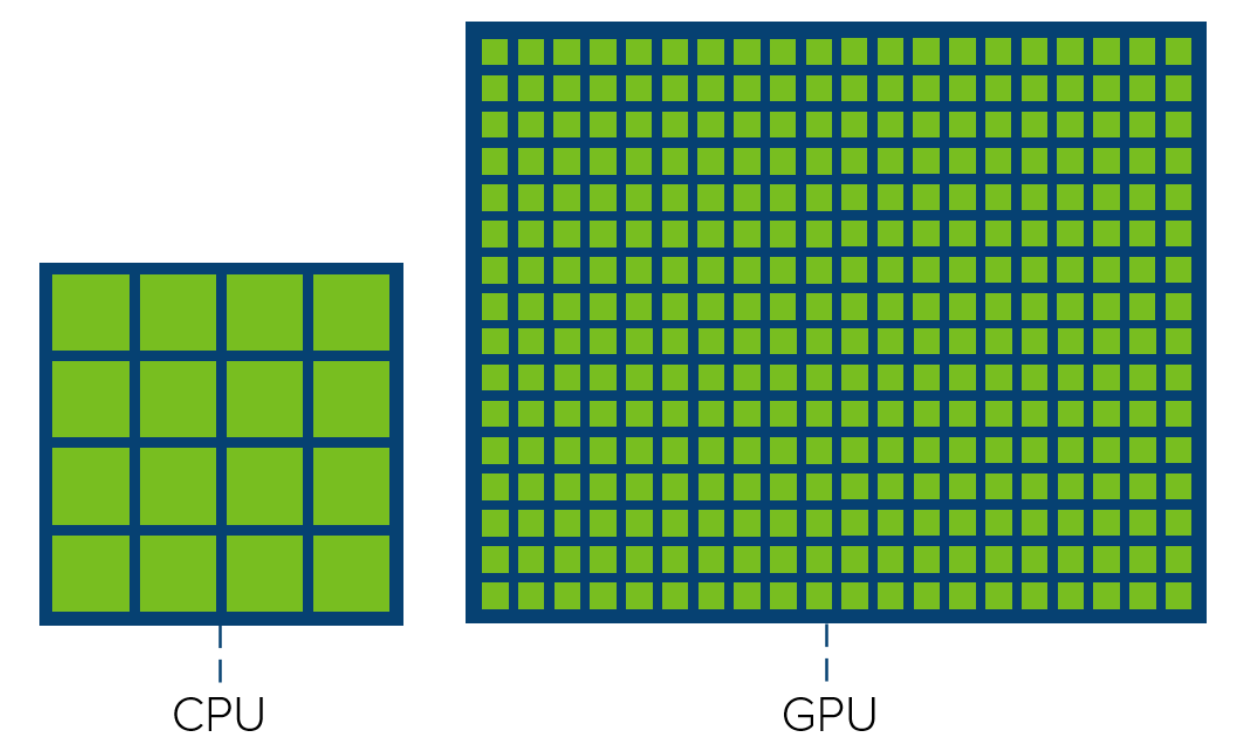
\includegraphics[width=0.4\textwidth]{images/cpuvgpu.png}
  \end{center}
\end{frame}

\begin{frame}{Limitations in JAX}
  \begin{itemize}
    \item Vectors length must be defined at compilation
  \end{itemize}
\end{frame}

\begin{frame}{Limitations in JAX}
  \begin{itemize}
    \item Vectors length must be defined at compilation
    \item Limited control flow (no while loops, etc)
  \end{itemize}
\end{frame}

\begin{frame}{Limitations in JAX}
  \begin{itemize}
    \item Vectors length must be defined at compilation
    \item Limited control flow (no while loops, etc)
    \item Debugging and optimising is hard
  \end{itemize}
\end{frame}

\begin{frame}[fragile]{JAX numpy vs numpy}
  \begin{columns}
    \column{0.5\textwidth}
    \begin{verbatim}
    import numpy as np
    x = np.arange(10)
    y = np.zeros_like(x)
    for i in range(len(x)):
        y[i] = x[i] * 2
    \end{verbatim}
    \column{0.5\textwidth}
    \begin{verbatim}
    import jax.numpy as jnp
    from jax import vmap
    x = jnp.arange(10)
    def double(v):
        return v * 2
    y = vmap(double)(x)
    \end{verbatim}
  \end{columns}
\end{frame}

\begin{frame}
\frametitle{What is JAX bandflux?}
\begin{columns}[c]
  \column{0.5\textwidth}
  \centering
  
\includegraphics[height=2cm]{images/sncosmobanner.png}
  \column{0.5\textwidth}
  \centering
  
\includegraphics[height=3cm]{images/jax_logo_250px.png}
\end{columns}
\vspace{1cm}
\begin{columns}
  \column{1\textwidth}
  \centering
  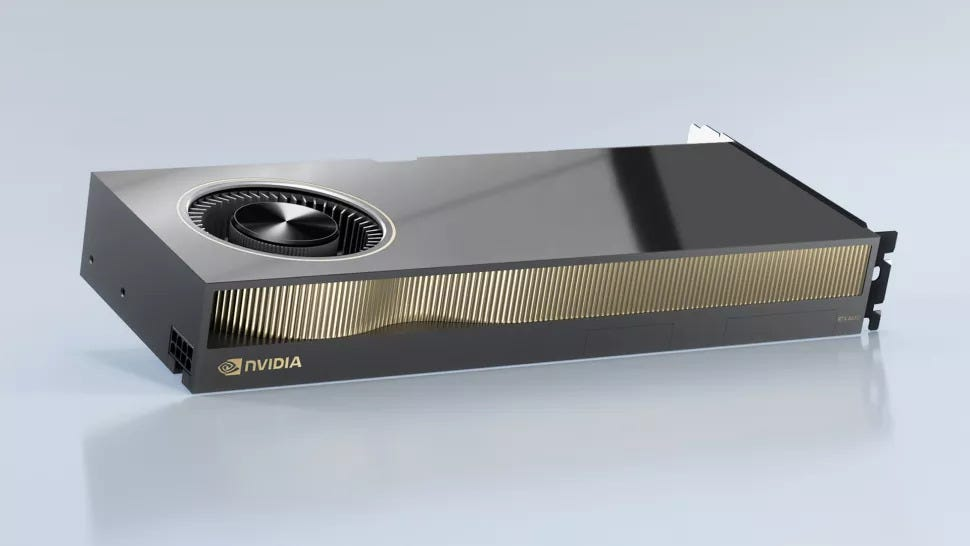
\includegraphics[height=3cm]{images/gpu.jpg}
\end{columns}
\end{frame}

\begin{frame}{What does JAX-bandflux do?}
  \begin{equation}
    F(p, \lambda) = x_0 \bigl[ M_0(p,\lambda) + x_1 M_1(p,\lambda) + \ldots \bigr] \times \exp\bigl[c \, CL(\lambda)\bigr]
  \end{equation}
  \begin{columns}
    \column{0.5\textwidth}
      \textbf{IN:}
      \begin{itemize}
        \item $x_0, x_1, t_0, c$
        \item $M_0(p,\lambda), M_1(p,\lambda)$
        \item $p$ (phase/redshift)
        \item $CL(\lambda)$
      \end{itemize}
    \column{0.5\textwidth}
      \textbf{OUT:}
      \begin{itemize}
        \item Flux: $F(p,\lambda)$
      \end{itemize}
  \end{columns}
\end{frame}

\begin{frame}{Bandflux Computation}
  \begin{itemize}
    \item Bandflux: Integrated flux through a specific filter
  \end{itemize}
  
  \begin{equation}
    \text{bandflux} = \int_{\lambda_\text{min}}^{\lambda_\text{max}} F(\lambda) \cdot T(\lambda) \cdot \frac{\lambda}{hc} \, d\lambda
  \end{equation}
  
  \begin{itemize}
    \item Components:
      \begin{itemize}
        \item $F(\lambda)$: Spectral flux density
        \item $T(\lambda)$: Filter transmission function
        \item $\lambda/(hc)$: Conversion from energy to photon counts
      \end{itemize}
    \item Implementation in JAX-bandflux:
      \begin{itemize}
        \item Vectorized array operations
        \item JIT-compiled for efficiency
        \item Trapezoidal integration along wavelength dimension
        \item Parallelized across multiple data instances via \texttt{vmap}
      \end{itemize}
  \end{itemize}
\end{frame}

\begin{frame}{Can now construct GPU compatible likelihood}
  \[
    \mathcal{L}(\mathbf{F}\mid\theta)
      = \prod_{i} \frac{1}{\sqrt{2\pi}\,\sigma_i}
        \exp\!\Bigg[-\frac{(F_i - \mu_i(\theta))^2}{2\,\sigma_i^2}\Bigg]
  \]
  \begin{itemize}
    \item Observed fluxes \(F_i\): measured data; model fluxes \(\mu_i(\theta)\): predicted flux given parameters
    \item With this likelihood we can now perform parameter estimation
    \item Likelihood is differentiable and can be compiled as part of broader GPU workflows
  \end{itemize}
\end{frame}

\begin{frame}{Can now fit light curves on GPU}
  \begin{center}
    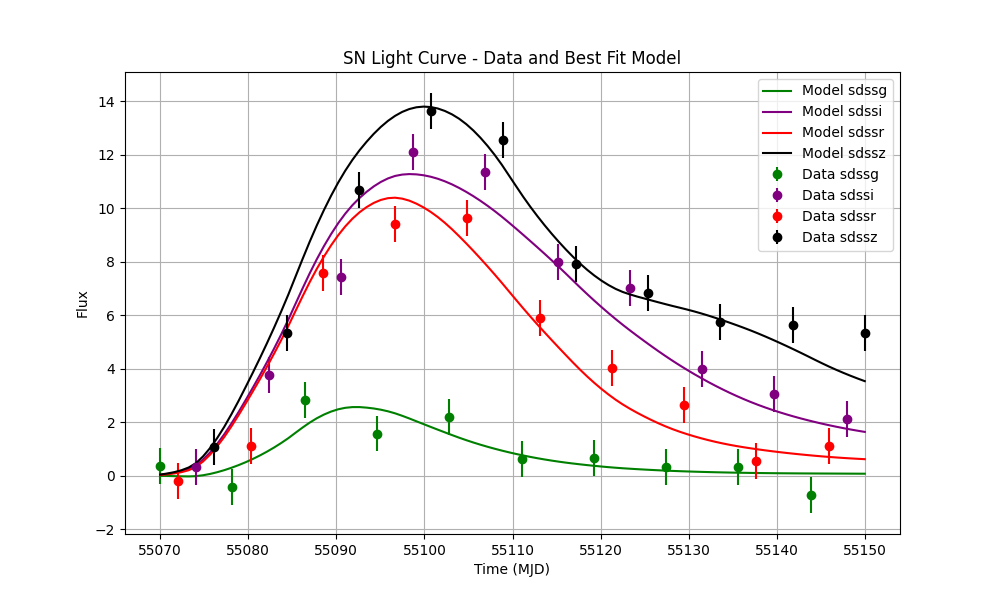
\includegraphics[width=0.8\textwidth]{images/sncosmo-fitter.png}
  \end{center}
\end{frame}


\begin{frame}{Bandflux Computation Example}
  \begin{itemize}
    \item For a detailed walkthrough of bandflux computation:
    \begin{itemize}
      \item Interactive Jupyter notebook with step-by-step implementation
      \item Demonstrates JAX-bandflux API usage
      \item Shows performance benefits of GPU acceleration
      \item Includes visualization of results
    \end{itemize}
    \item Access the example notebook:
    \begin{center}
      \href{https://github.com/handley-lab/nested-sampling-book/blob/main/physics/supernovae.ipynb}{Supernovae Analysis Example Notebook}
    \end{center}
  \end{itemize}
\end{frame}
\begin{frame}{PIP installable}
  \vfill
  \begin{center}
    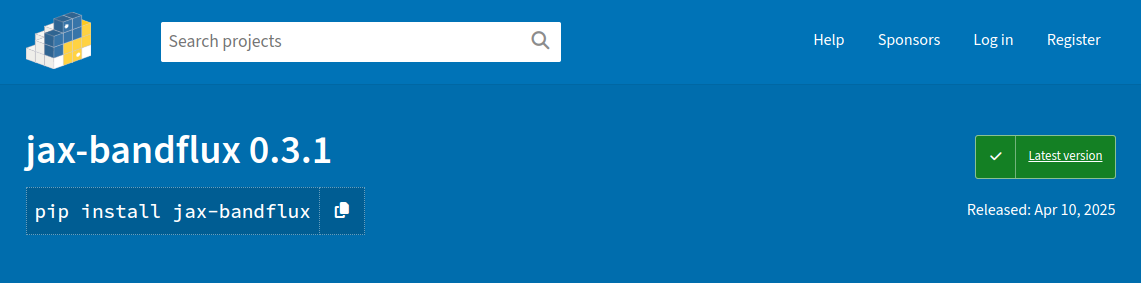
\includegraphics[width=0.8\textwidth]{images/jaxbandflux-pip.png}
  \end{center}
  \vfill
  \begin{center}
    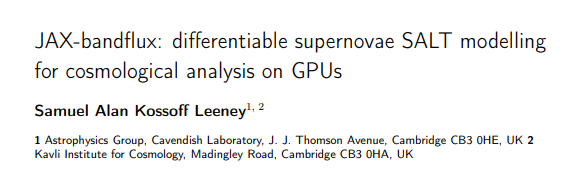
\includegraphics[width=0.8\textwidth]{images/jaxbandflux-paper.png}
  \end{center}
  \vfill
\end{frame}

\section{Bayesian anomaly detection}

\begin{frame}{Over simplified example of anomaly detection method (thresholding)}
  \footnotesize
  \textbf{Simple statistical approach:}
  \begin{itemize}
    \item Calculate mean ($\mu$) and standard deviation ($\sigma$) of the data
    \item Define threshold $T = \mu + k\sigma$ where $k$ is a sensitivity parameter
    \item Flag data point $x_i$ as anomalous if:
  \end{itemize}
  \begin{equation}
    \text{anomaly}_i = \begin{cases}
      1 & \text{if } x_i > T \\
      0 & \text{otherwise}
    \end{cases}
  \end{equation}
  \textbf{Limitations:}
  \begin{itemize}
    \item Choice of $k$ is arbitrary
    \item Assumes Gaussian statistics
    \item No consideration of temporal correlations
    \item Cannot distinguish between RFI and real signals
  \end{itemize}
\end{frame}

\begin{frame}{Thresholding results}
  \begin{columns}
    \column{0.5\textwidth}
    \textbf{Constant signal with RFI:}
    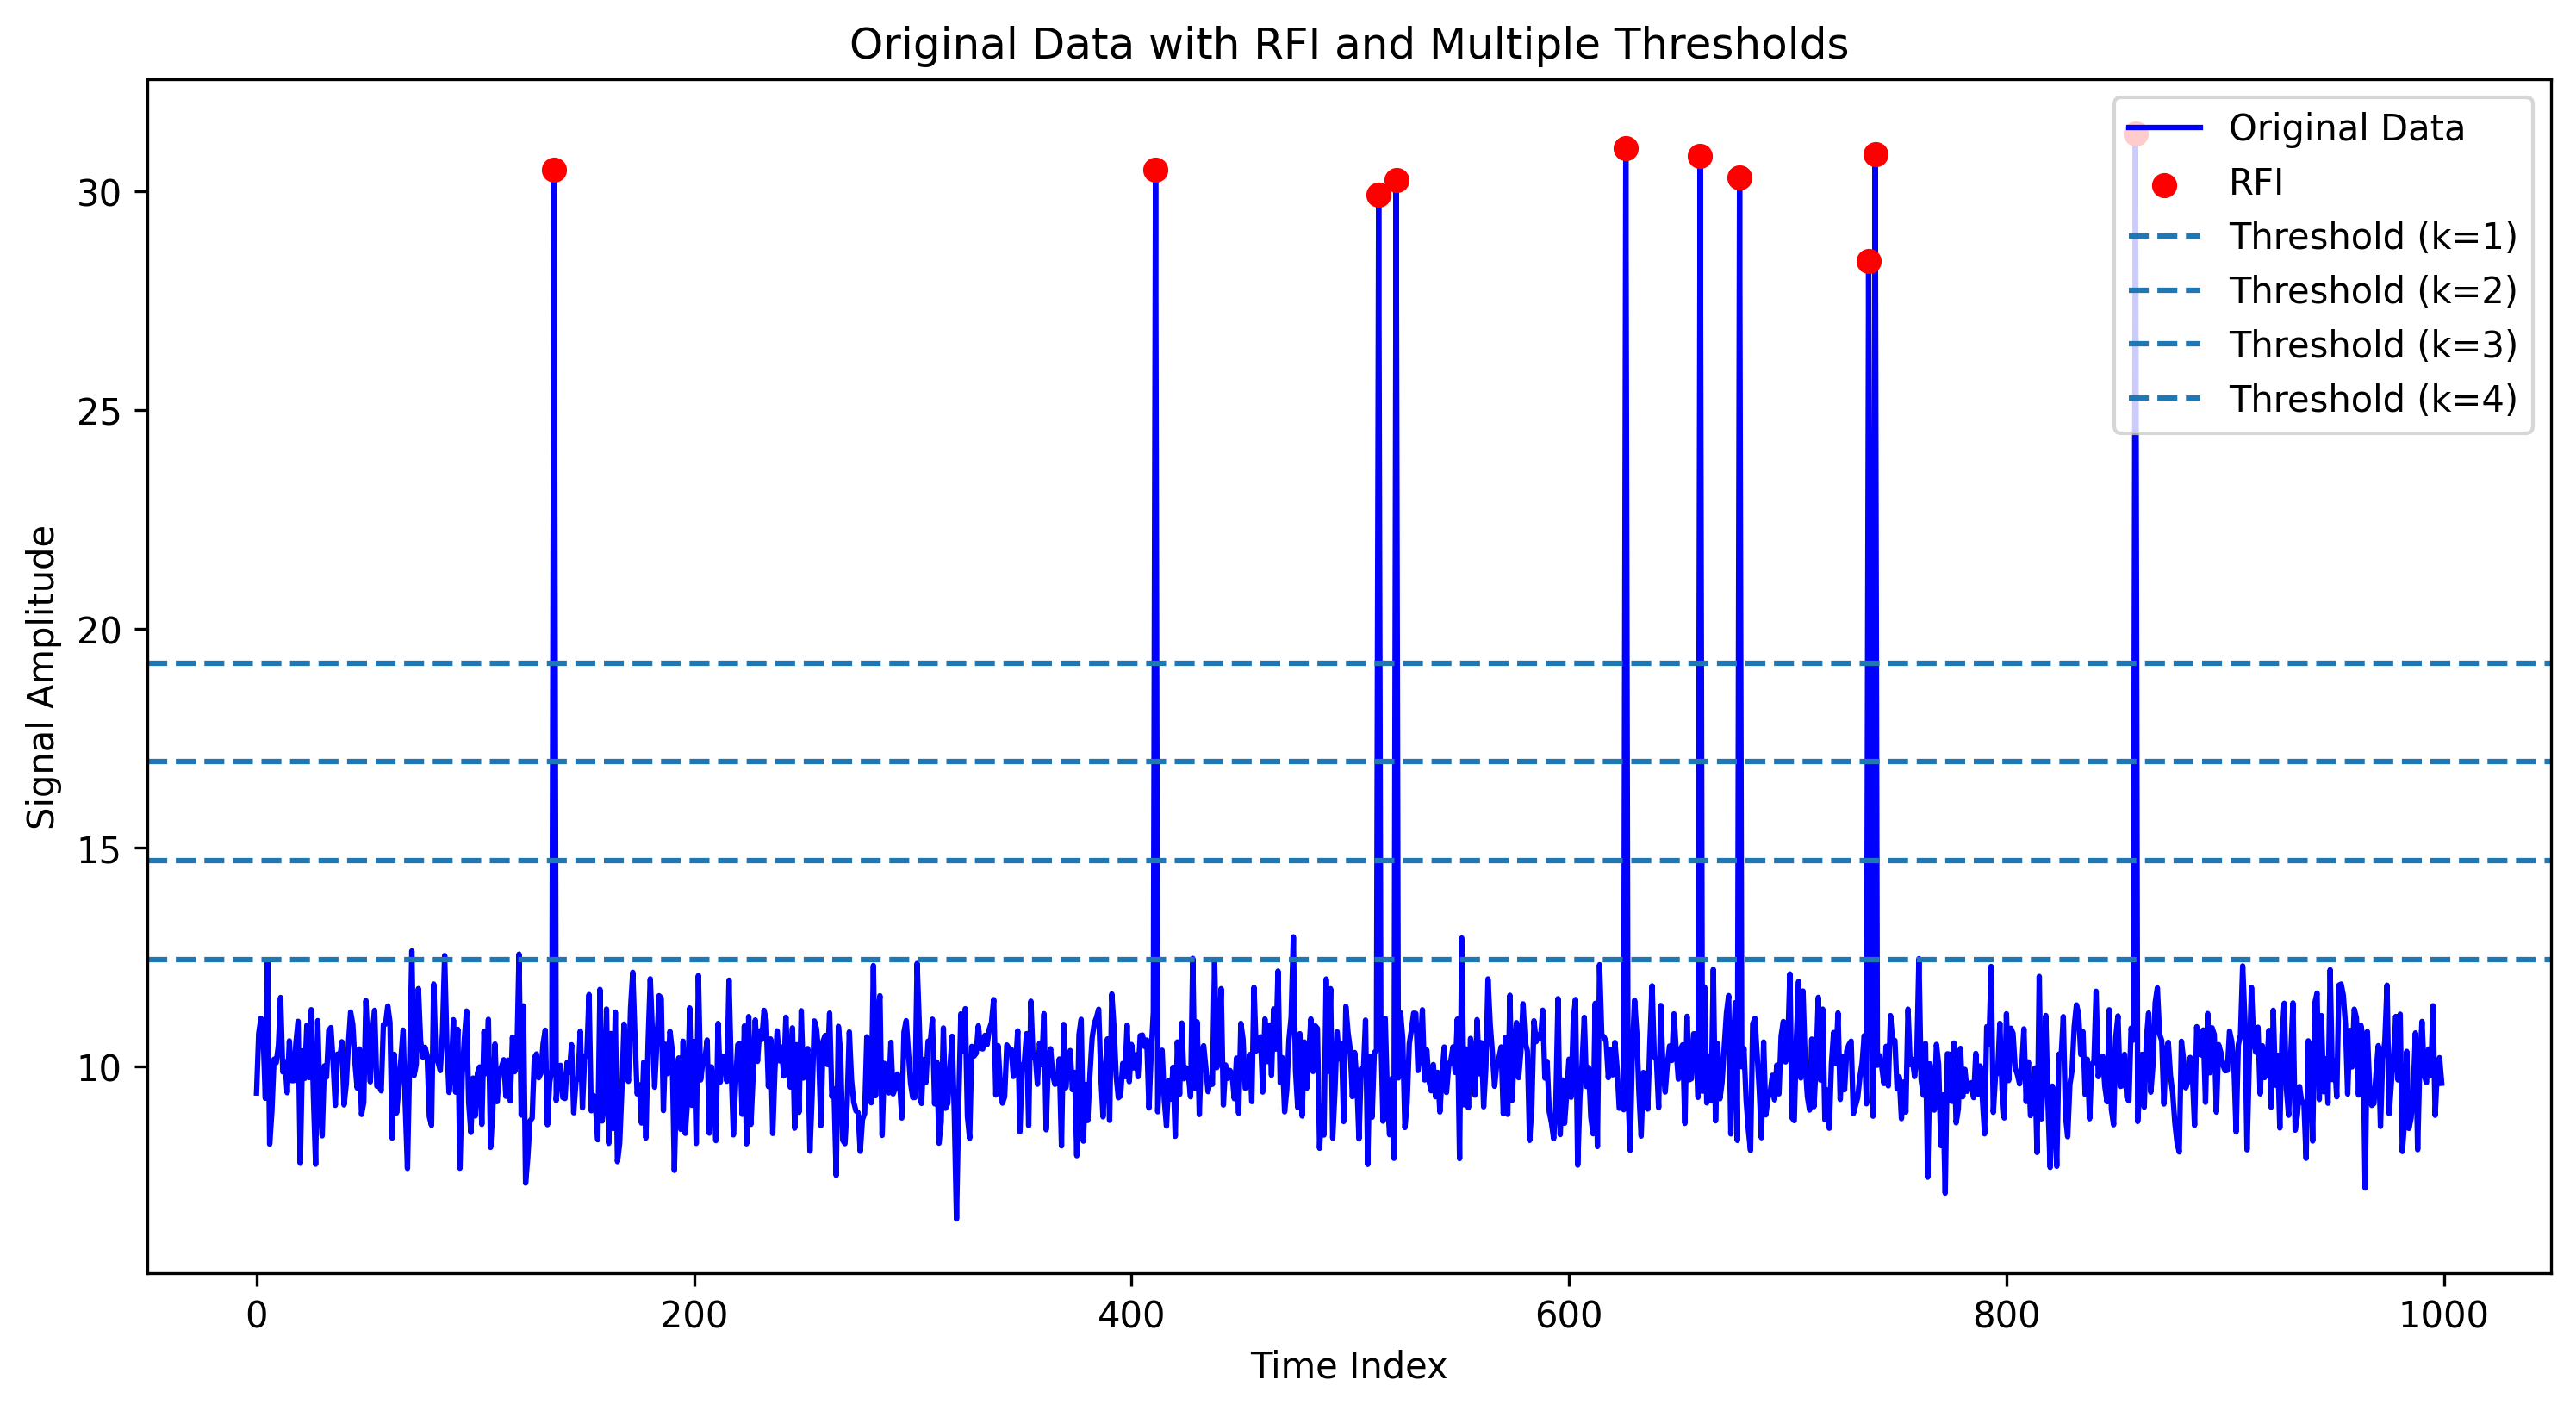
\includegraphics[width=\textwidth]{images/threshold_multiple.png}
    \column{0.5\textwidth}
    \textbf{Sine wave with RFI:}
    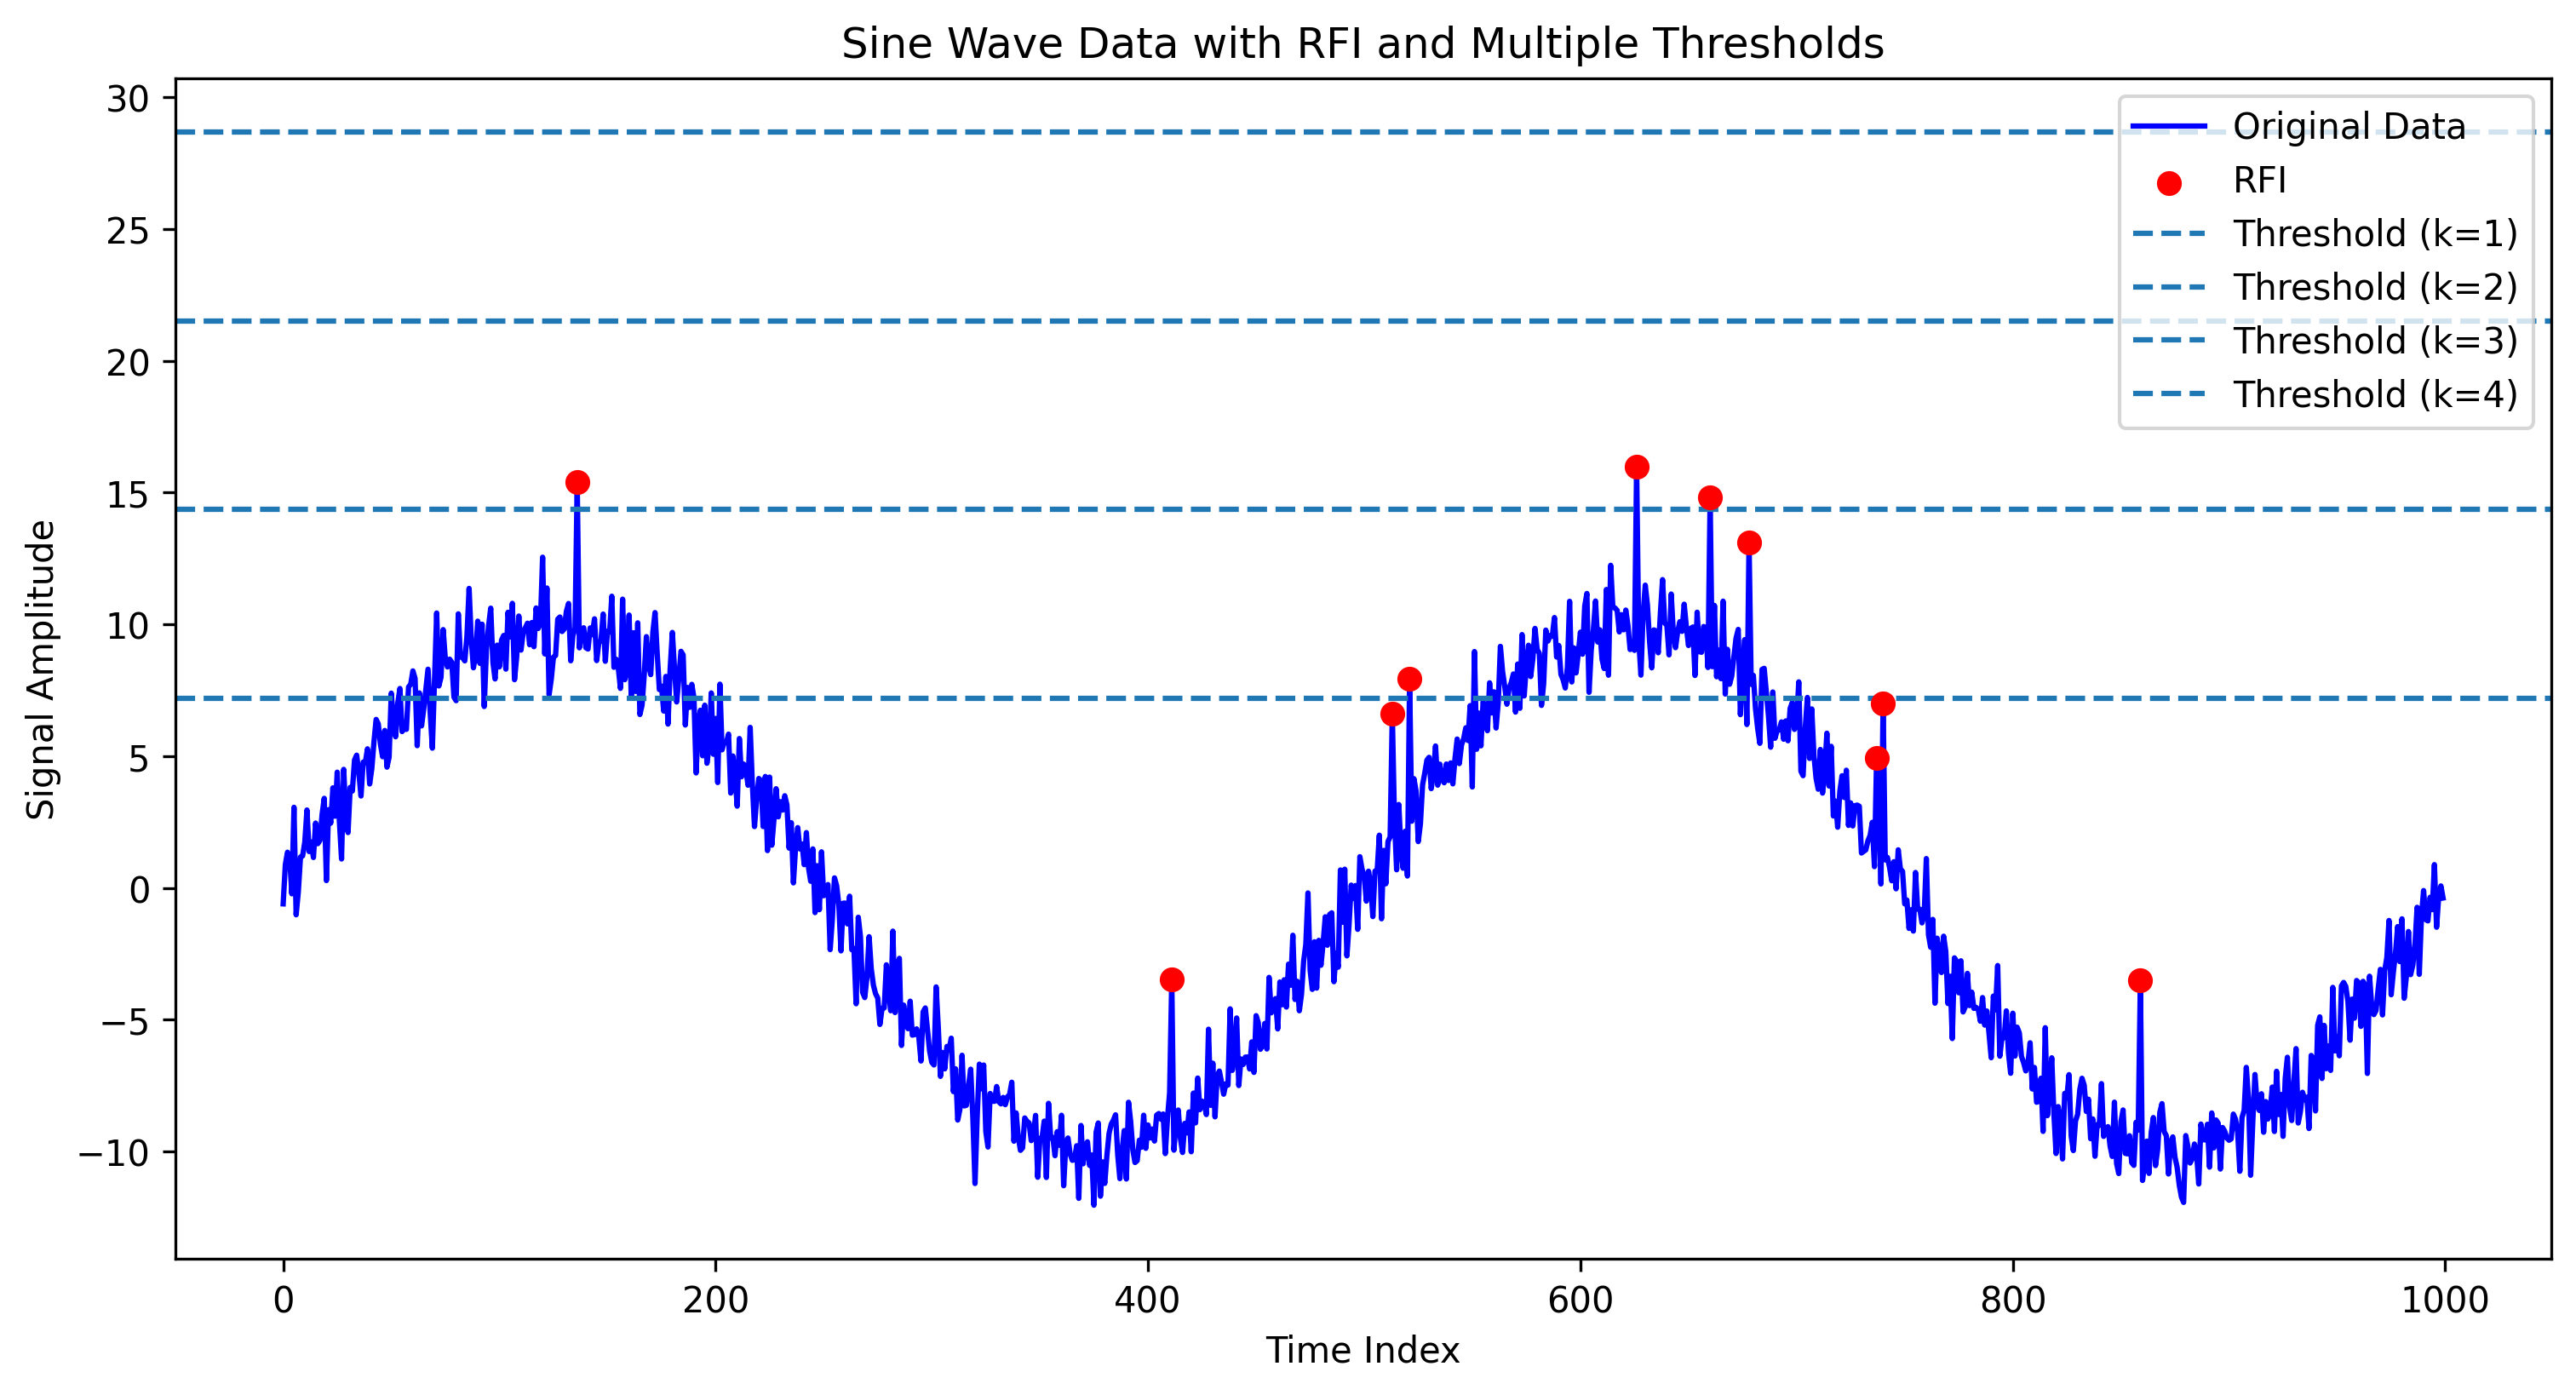
\includegraphics[width=\textwidth]{images/threshold_sin_multiple.png}
  \end{columns}
\end{frame}

\begin{frame}{Defining an anomaly sensitive likelihood}
  \footnotesize
  \textbf{a) Generate peicewise likelihood:}
  \begin{equation}
      P(\mathcal{D}_i|\theta) = \begin{cases}
          \mathcal{L}_i(\theta) &: \text{expected}\\
          \Delta^{-1}[ 0<\mathcal{D}_i<\Delta] &: \text{anomalous},
      \end{cases}
  \end{equation}

  \textbf{b) Ascribe Bernoulli prior:}
  \begin{equation}
      P(\varepsilon_i) = p^{(1-\varepsilon_i)}(1-p)^{\varepsilon_i}.
  \end{equation}

  \textbf{c) Marginalise over epsilon:}
  \begin{equation}
      P(\mathcal{D} | \theta) =\sum_{\varepsilon \in \{ 0, 1 \} ^N}P(\mathcal{D},\varepsilon|\theta)
    \end{equation}


    \textbf{d) Approximate correct mask is most likely}
     \begin{equation}
 P(\mathcal{D}|\theta, \varepsilon_{\mathrm{max}}) \gg \mathrm{max}_j P(\mathcal{D}|\theta,\varepsilon^{(j)})\label{eq:nlo},
\end{equation}

  \textbf{e) Loglikelihood:}
  \begin{equation}
      \log{P(\mathcal{D}|\theta)} = \sum_{i}[{\log{\mathcal{L}_i}+\log({1-p})]\varepsilon^{\mathrm{max}}_i + [\log{p} - \log{\Delta}](1 - \varepsilon^\mathrm{max}_i})
  \end{equation}
\end{frame}

\begin{frame}{Computing the Posterior}
    \footnotesize
    \textbf{e) Loglikelihood:}
  \begin{equation}\tag{6}
      \log{P(\mathcal{D}|\theta)} = \sum_{i}[{\log{\mathcal{L}_i}+\log({1-p})]\varepsilon^{\mathrm{max}}_i + [\log{p} - \log{\Delta}](1 - \varepsilon^\mathrm{max}_i})
  \end{equation}

    \footnotesize
    \textbf{f) Maximise $\varepsilon^{max}$ by comparing the terms:}
    \begin{equation}\tag{7}
    \log P(\mathcal{D}|\theta) =
    \begin{cases}
    \log \mathcal{L}_i + \log(1 - p), & \text{if } [\log \mathcal{L}_i + \log(1 - p) > \log p - \log \Delta] \\
    \log p - \log \Delta, & \text{otherwise}
    \end{cases}
    \end{equation}
\end{frame}

\begin{frame}{Fit on a simple toy model}
    \centering
    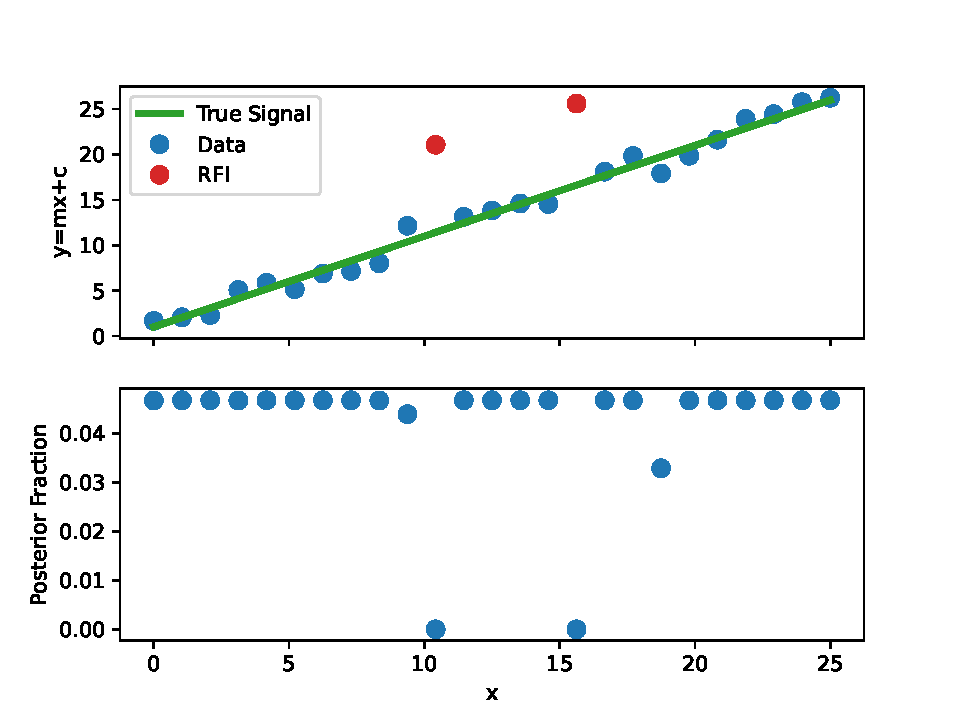
\includegraphics[width=0.7\textwidth]{images/test.pdf}
  \end{frame}

\begin{frame}{Likelihood thresholding condition $p$}
    \begin{equation}
    \begin{aligned}
    \log{P(\mathcal{D}|\theta)} &= \sum_{i}[{\log{\mathcal{L}_i}+\log({1-p})]\varepsilon^{\mathrm{max}} + [\log{p} - \log{\Delta}](1 - \varepsilon^\mathrm{max}_i})\label{eq:loglikelihood}
    \end{aligned}
    \end{equation}
    \centering
    \animategraphics[autoplay,loop,width=11cm]{2}{images/gif_anest/comb_}{1}{9}
\end{frame}

\begin{frame}{Varying $p$}
    \centering
    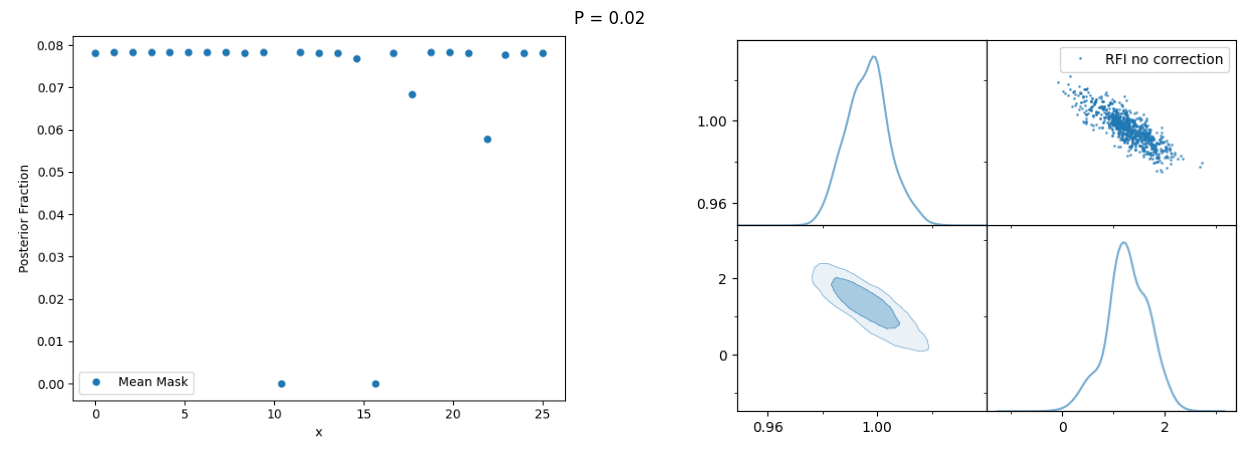
\includegraphics[width=\textwidth]{images/gif_anest/comb_2.png}
\end{frame}

\begin{frame}{Varying $p$}
    \centering
    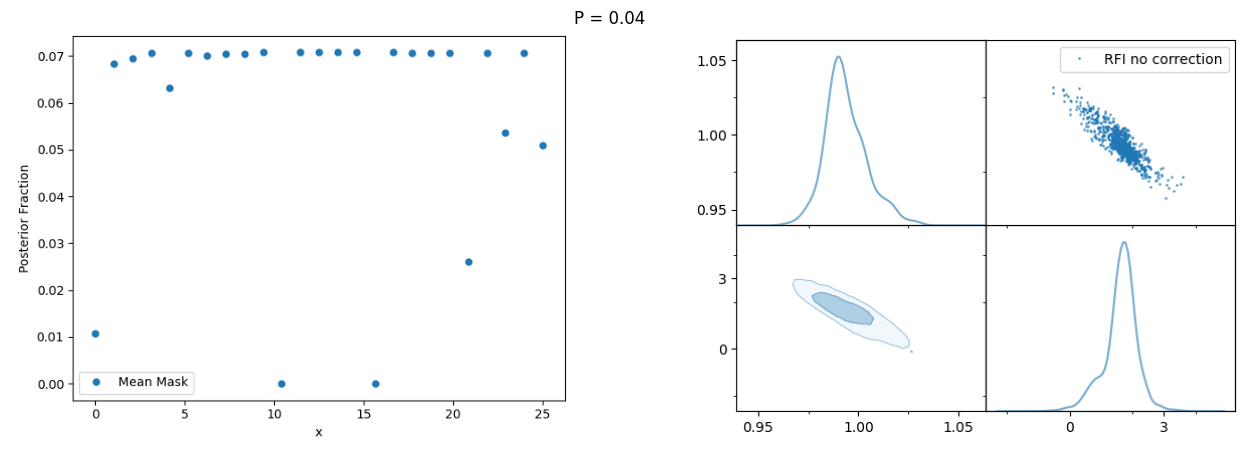
\includegraphics[width=\textwidth]{images/gif_anest/comb_3.png}
\end{frame}

\begin{frame}{Varying $p$}
    \centering
    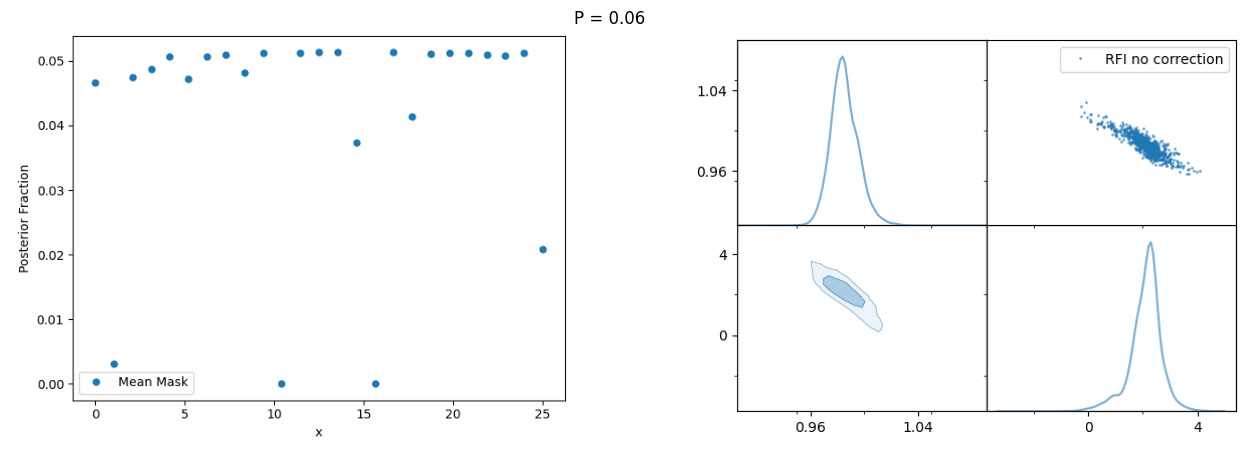
\includegraphics[width=\textwidth]{images/gif_anest/comb_4.png}
\end{frame}

\begin{frame}{Varying $p$}
    \centering
    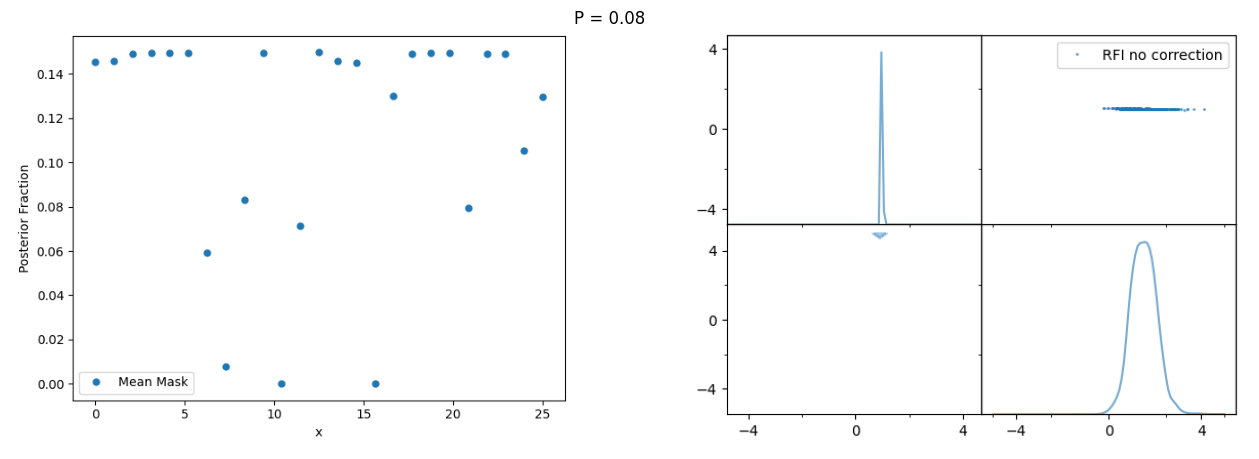
\includegraphics[width=\textwidth]{images/gif_anest/comb_5.png}
\end{frame}

\begin{frame}{Varying $p$}
    \centering
    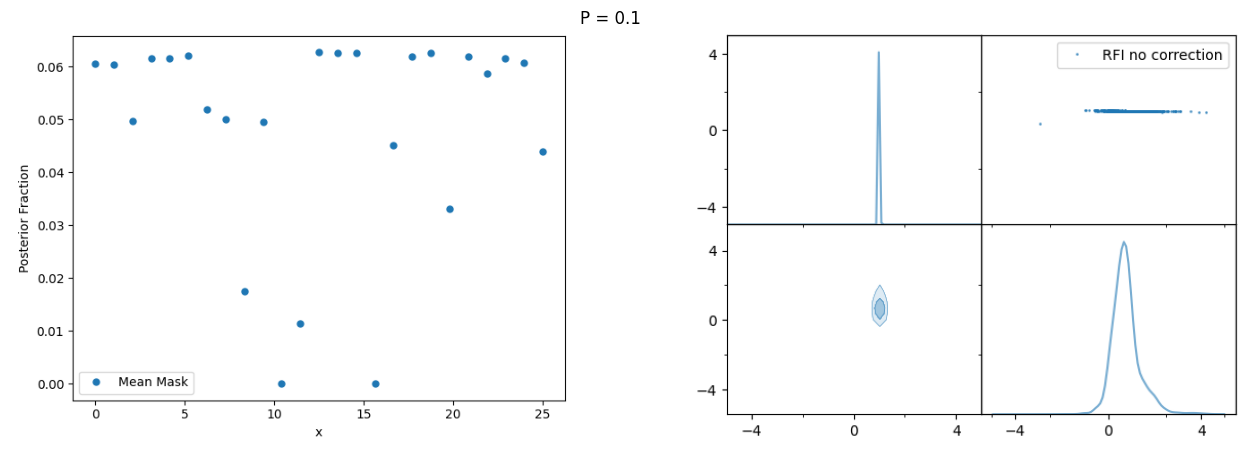
\includegraphics[width=\textwidth]{images/gif_anest/comb_6.png}
\end{frame}

\begin{frame}{Varying $p$}
    \centering
    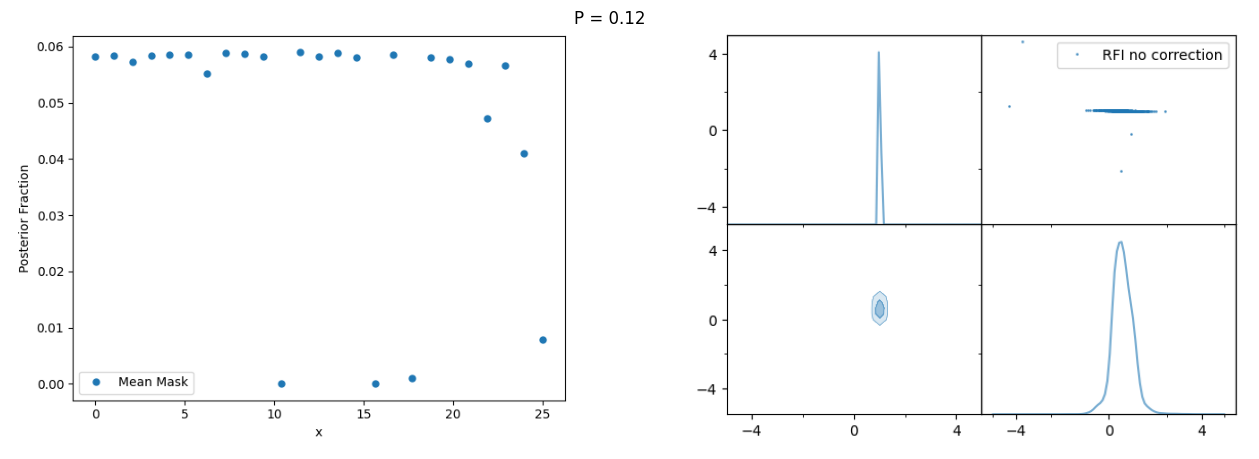
\includegraphics[width=\textwidth]{images/gif_anest/comb_7.png}
\end{frame}

\begin{frame}{Varying $p$}
    \centering
    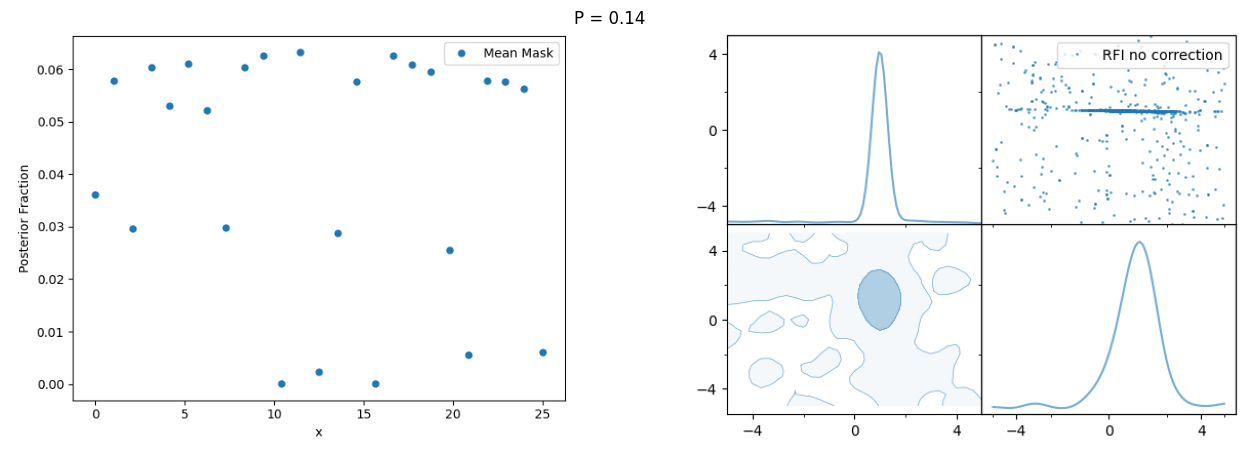
\includegraphics[width=\textwidth]{images/gif_anest/comb_8.png}
\end{frame}

\begin{frame}{Varying $p$}
    \centering
    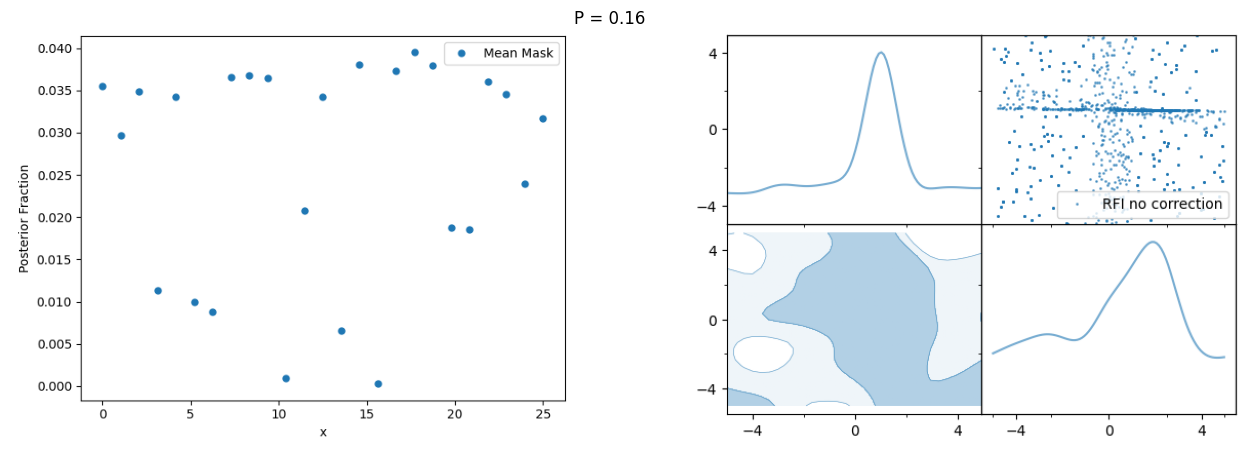
\includegraphics[width=\textwidth]{images/gif_anest/comb_9.png}
\end{frame}

\begin{frame}{Selection strategy for $p$.}
  \begin{columns}
    \column{0.5\textwidth}
    \begin{itemize}
      \item `Select $p$ such that the Bayesian evidence is maximised'
    \end{itemize}
    \column{0.5\textwidth}
    \begin{figure}
      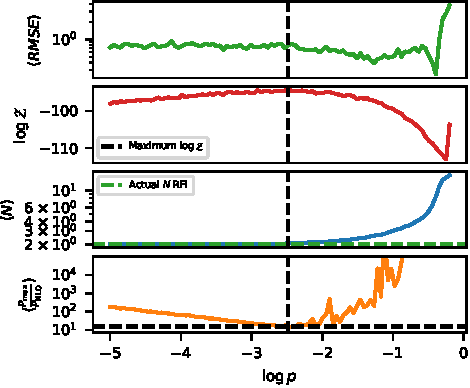
\includegraphics[width=1\textwidth]{images/f_approx_current_sig5_2.pdf}
    \end{figure}
  \end{columns}
\end{frame}


\begin{frame}{Fully automated anomaly detection}
  \begin{itemize}
  \item Putting a prior on $p$, we can fit it dynamically as a free parameter.
  \item This fully automates the anomaly detection process.
  \item Must exclude $p=0$.
  \end{itemize}
\end{frame}

\begin{frame}{Application to toy model}
  \centering
  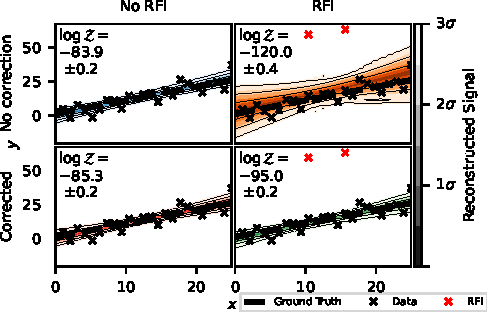
\includegraphics[width=0.8\textwidth]{images/4pane_toy_sidebar.pdf}
\end{frame}

\begin{frame}{Implement with 2 lines of code}
  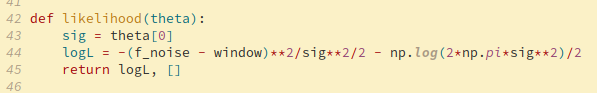
\includegraphics[width=1\textwidth]{images/logl1.png}
  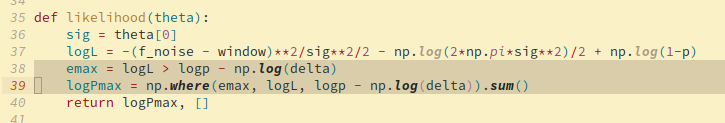
\includegraphics[width=1\textwidth]{images/logl2.png}
  \centering Tutorial @ github.com/samleeney
\end{frame}

\begin{frame}{Read the paper!}
  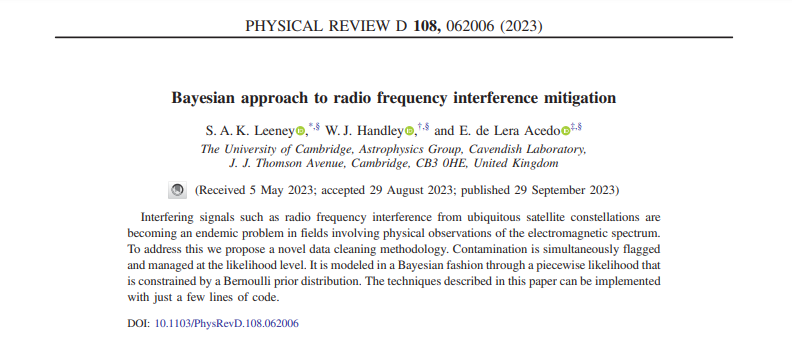
\includegraphics[width=1\textwidth]{images/paper1.png}
  \href{https://arxiv.org/abs/2211.15448}{arxiv: 2211.15448}
\end{frame}

\section{Apply on Ia supernovae}

\begin{frame}{Standard vs. Anomaly Detection Likelihoods}
  \begin{columns}
    \column{0.5\textwidth}
    \textbf{Standard Likelihood:}
    \begin{align}
      \log \mathcal{L}_{\text{std}} &= -\frac{1}{2}\sum_i \left(\frac{f_i - m_i}{\sigma_i}\right)^2 \nonumber \\
      &- \frac{1}{2}\sum_i \log(2\pi\sigma_i^2)
    \end{align}
    \begin{itemize}
      \item $f_i$: Observed flux
      \item $m_i$: Model flux (SALT3)
      \item $\sigma_i$: Flux uncertainty
    \end{itemize}
    
    \column{0.5\textwidth}
    \textbf{Anomaly Detection Likelihood:}
    \begin{align}
      \log \mathcal{L}_{\text{anom}} &= \sum_i \begin{cases}
        \log \mathcal{L}_i + \log(1-p), & \text{if } e_i^{\max} \\
        \log p - \log \Delta, & \text{otherwise}
      \end{cases}
    \end{align}
    \begin{itemize}
      \item $\log \mathcal{L}_i$: Point-wise standard likelihood
      \item $p$: Anomaly probability (fitted parameter)
      \item $e_i^{\max}$: Boolean indicating normal data
      \item $\Delta$: Maximum flux range
    \end{itemize}
  \end{columns}
  
\end{frame}
\begin{frame}{Applying to Ia supernovae}
\begin{center}
  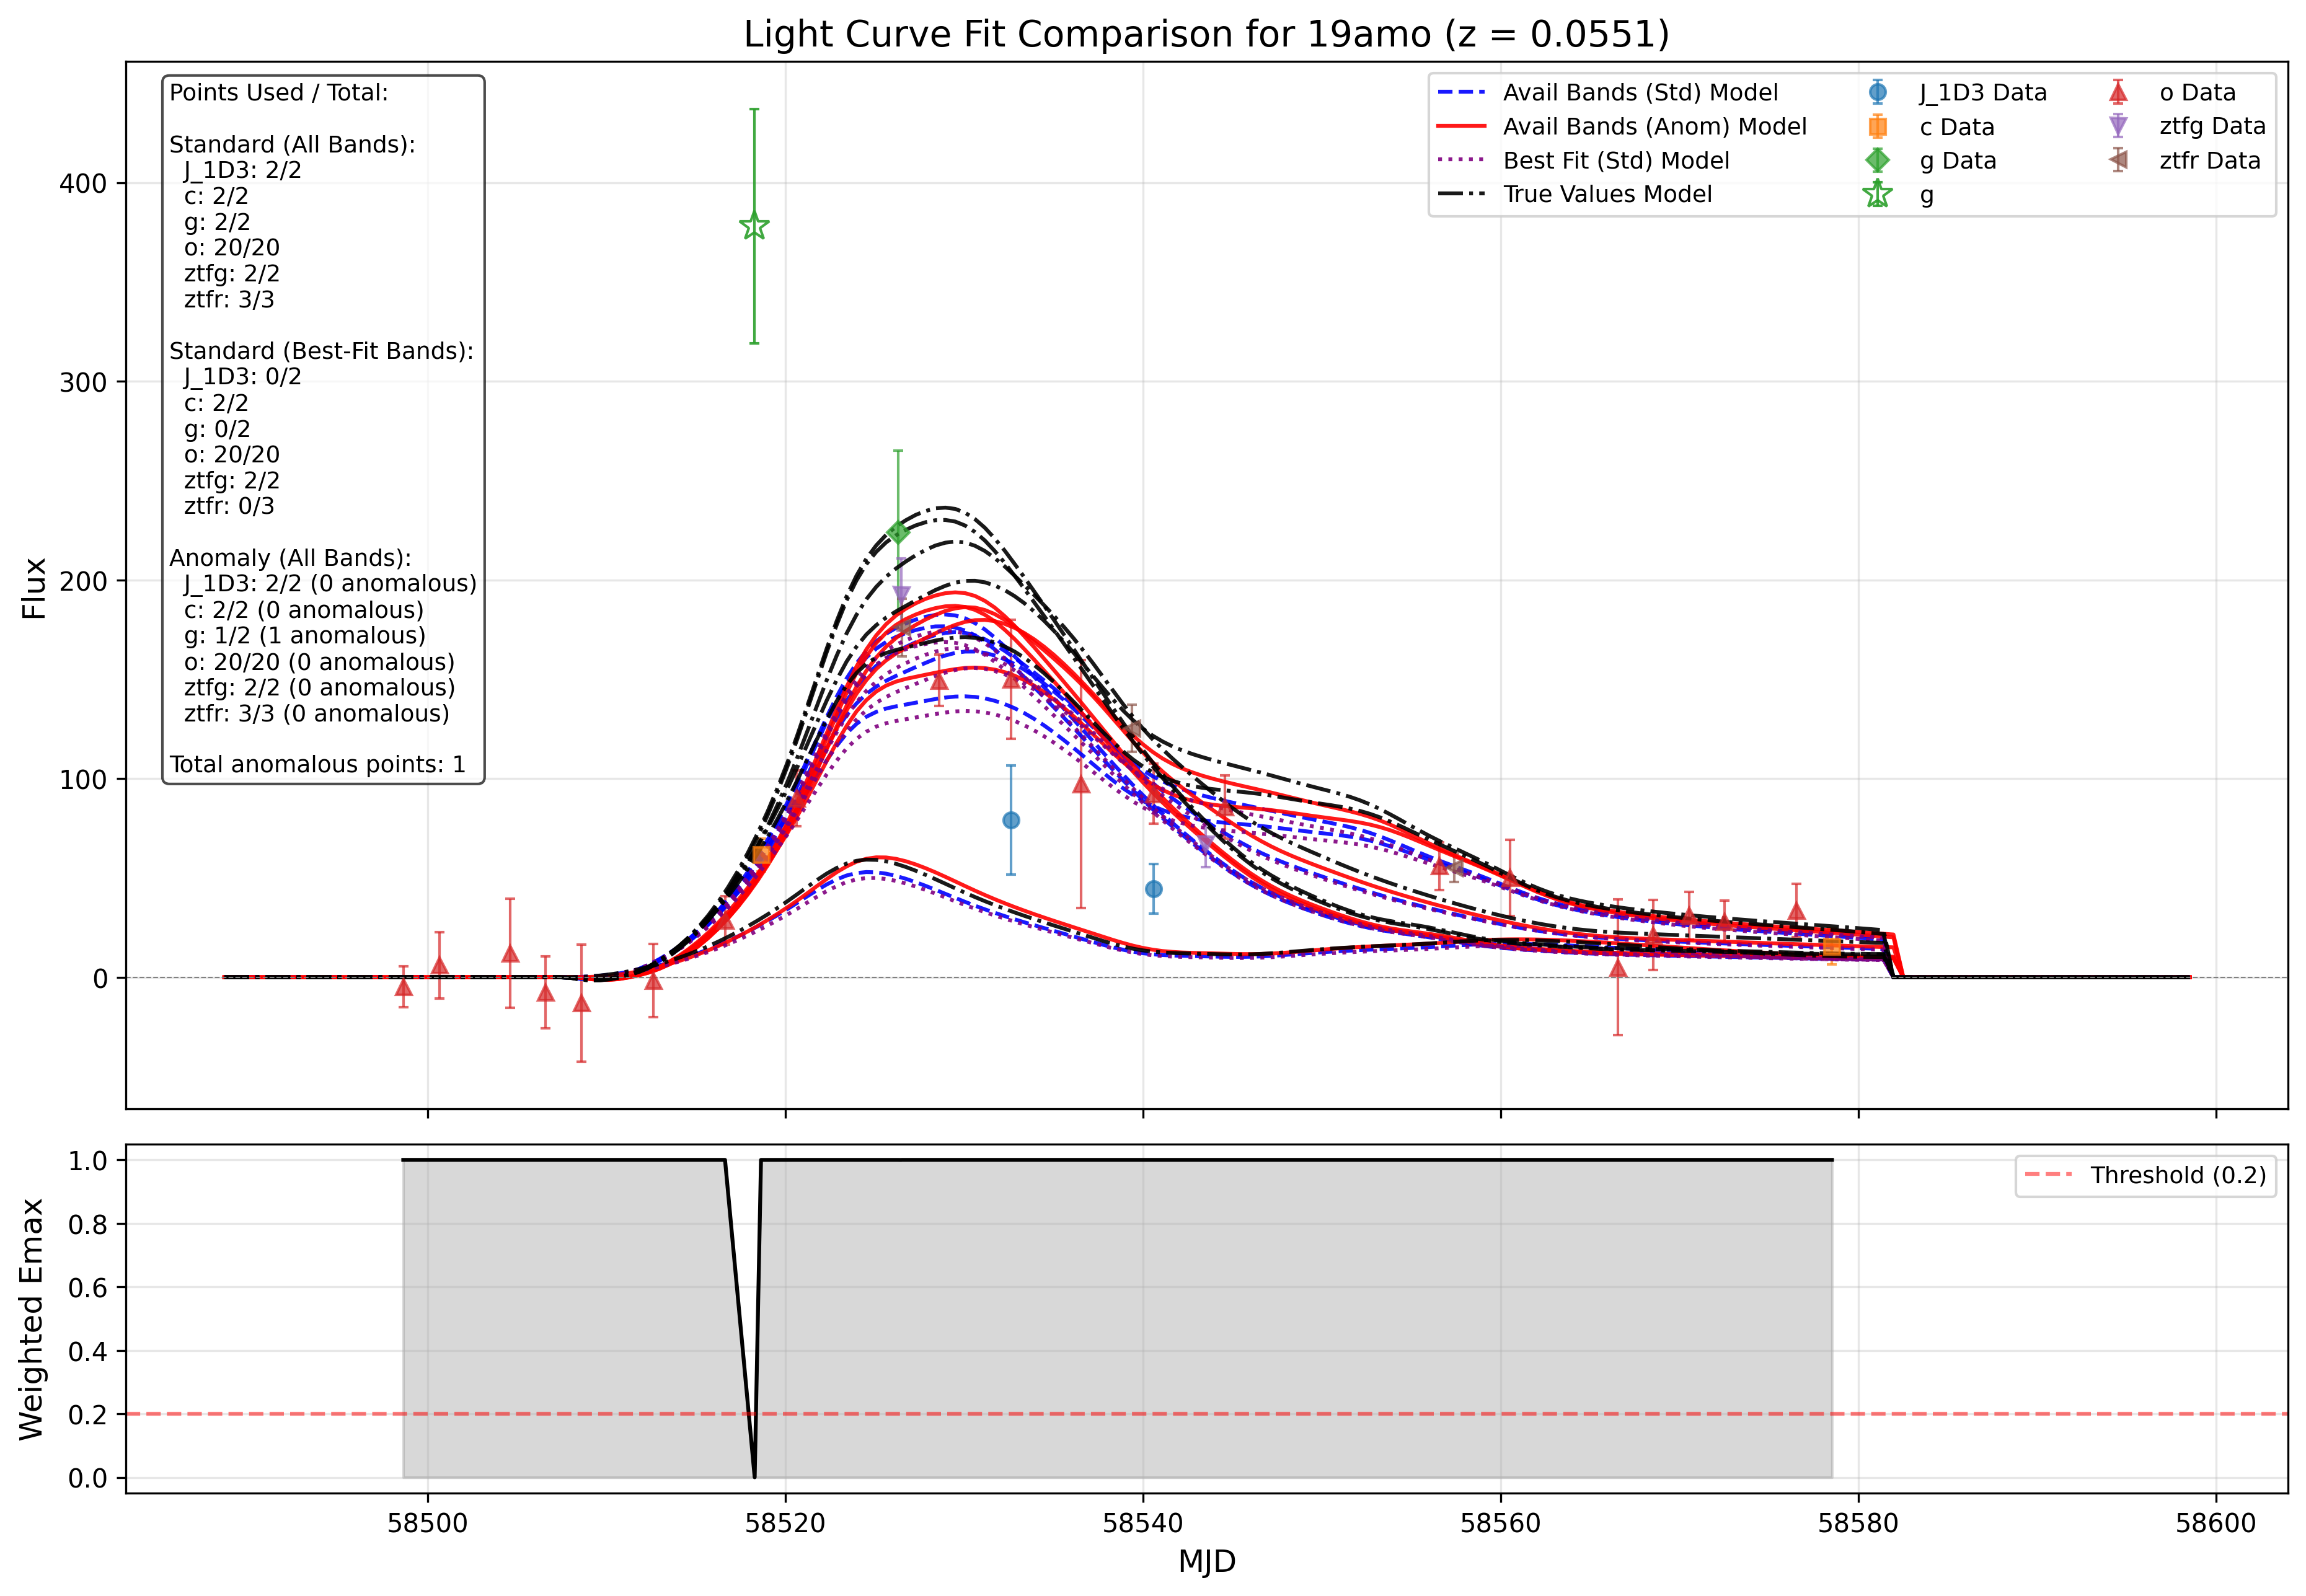
\includegraphics[width=0.8\textwidth]{images/light_curve_comparison_19amo.png}
\end{center}
\end{frame}



\begin{frame}{SN 19amo: Classic 'anomaly detection' example}
  \begin{columns}
    \column{0.5\textwidth}
    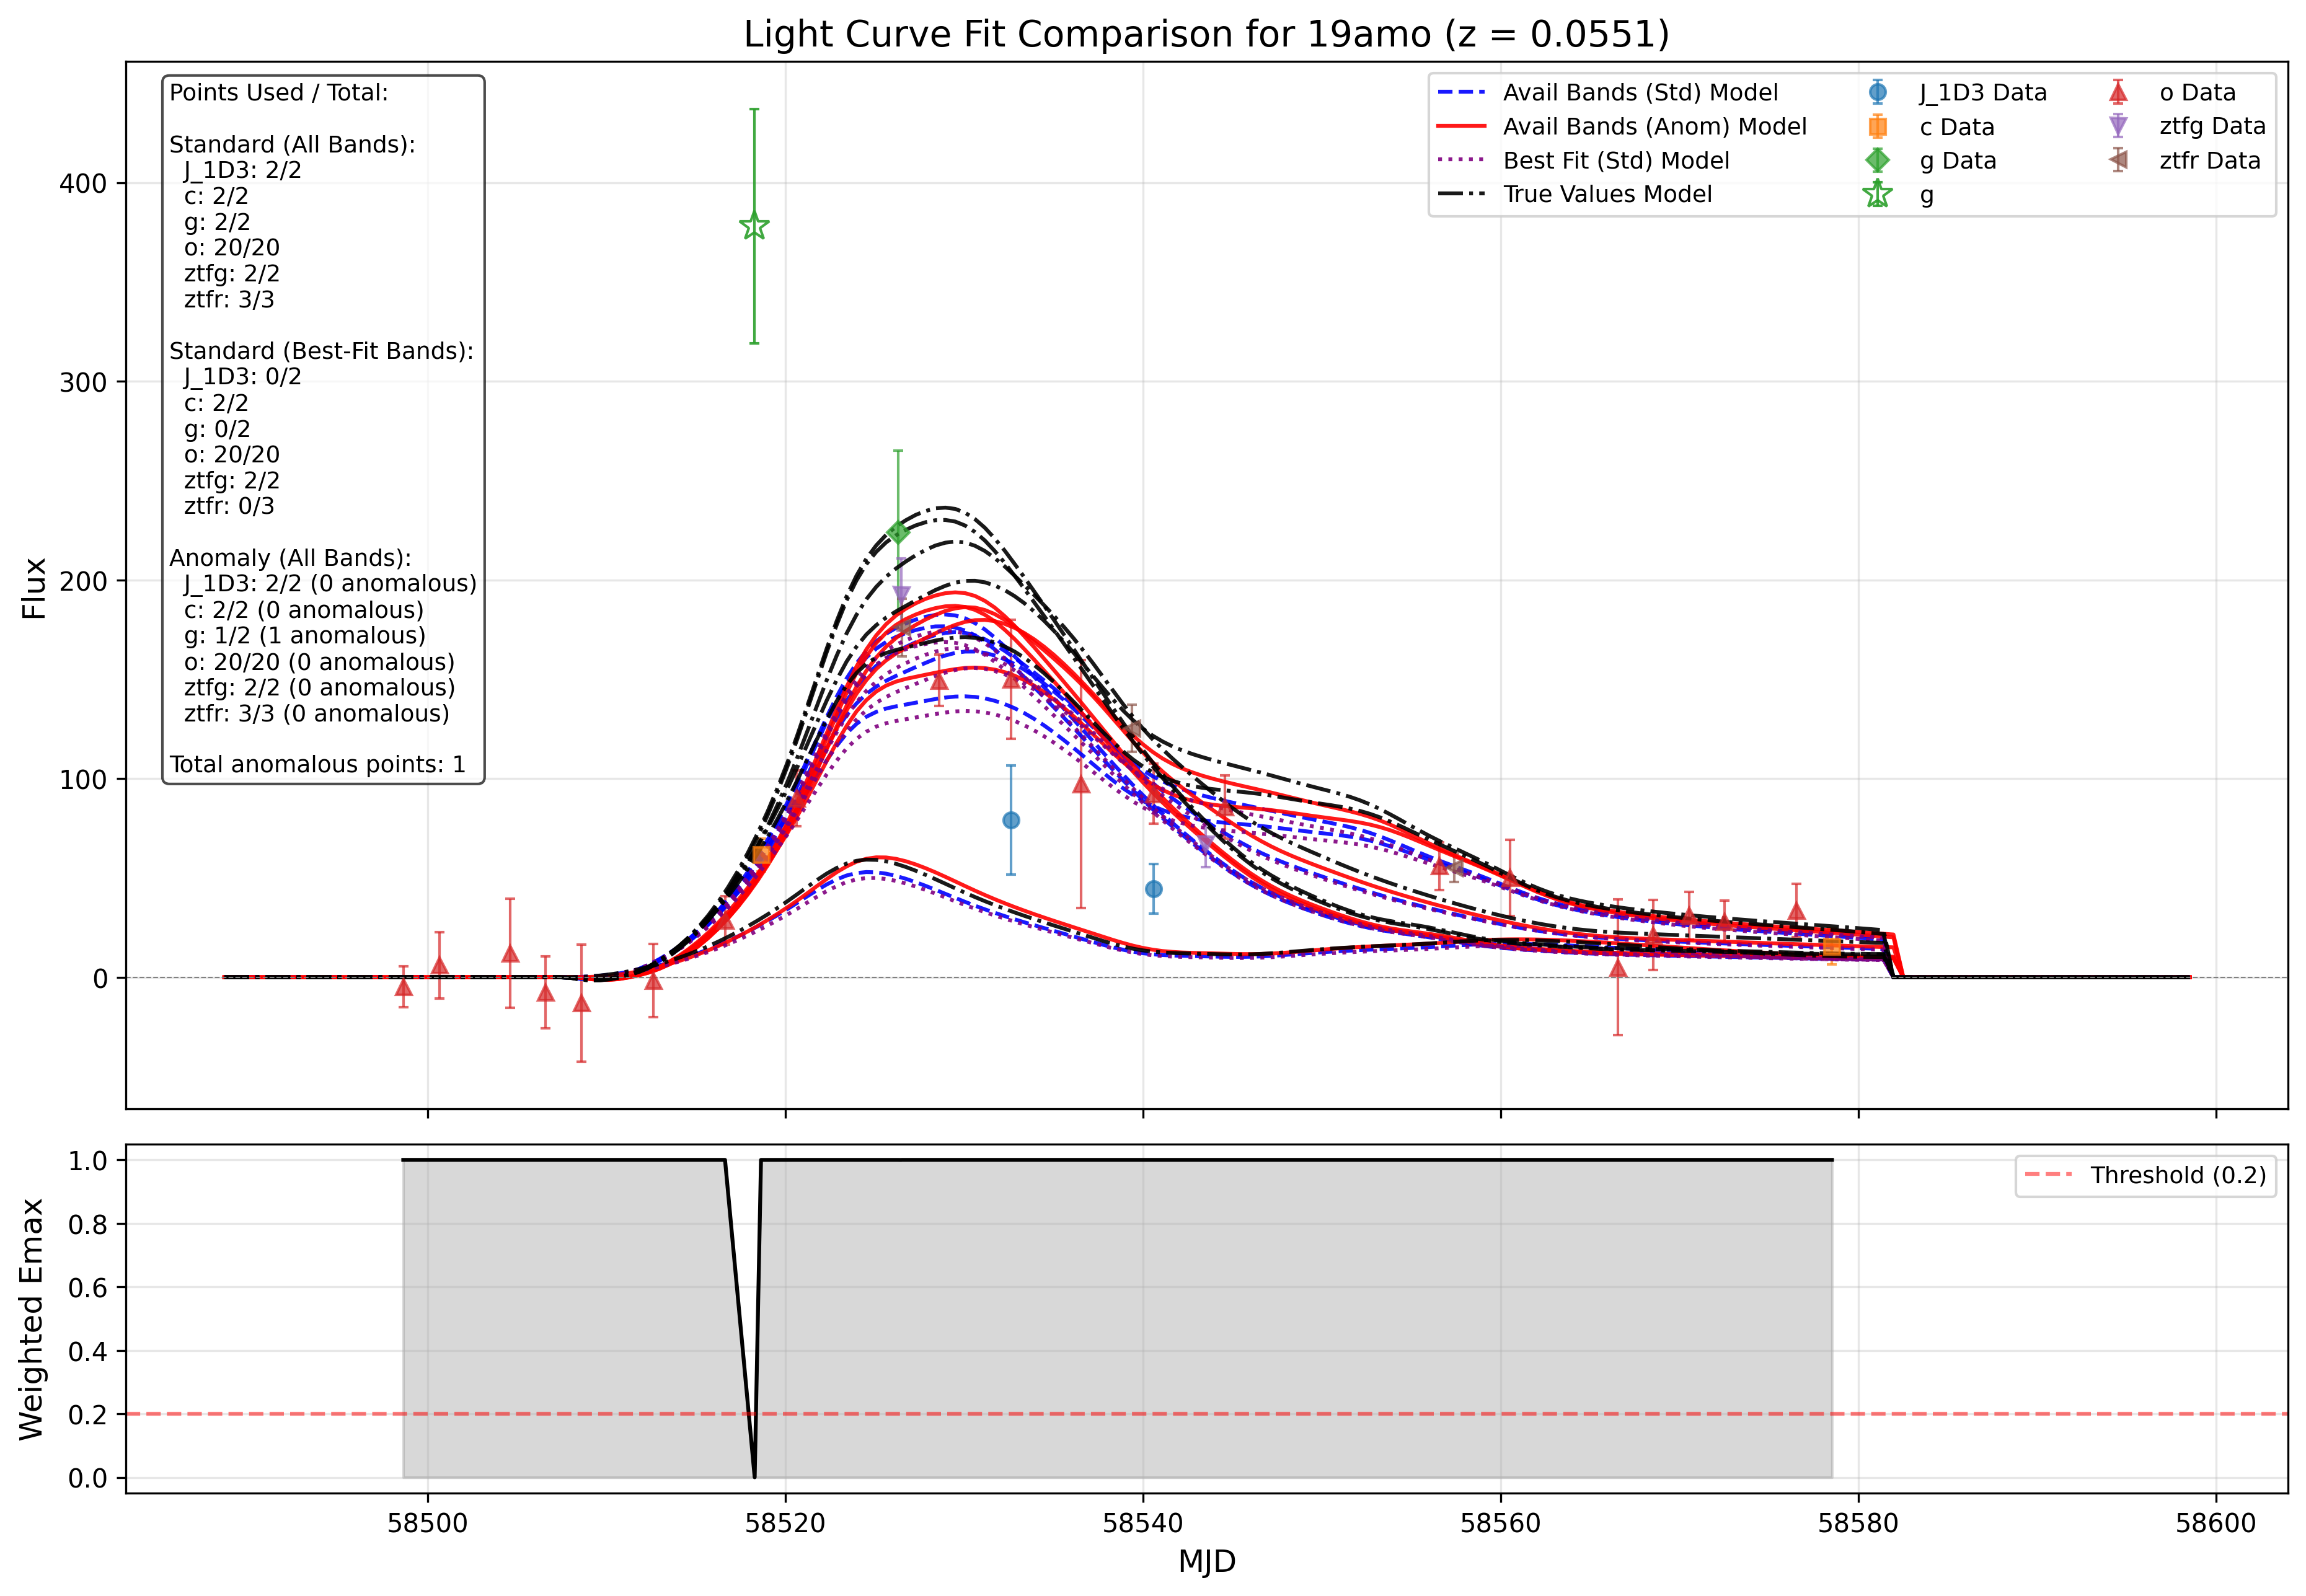
\includegraphics[width=\textwidth]{images/light_curve_comparison_19amo.png}
    \column{0.5\textwidth}
    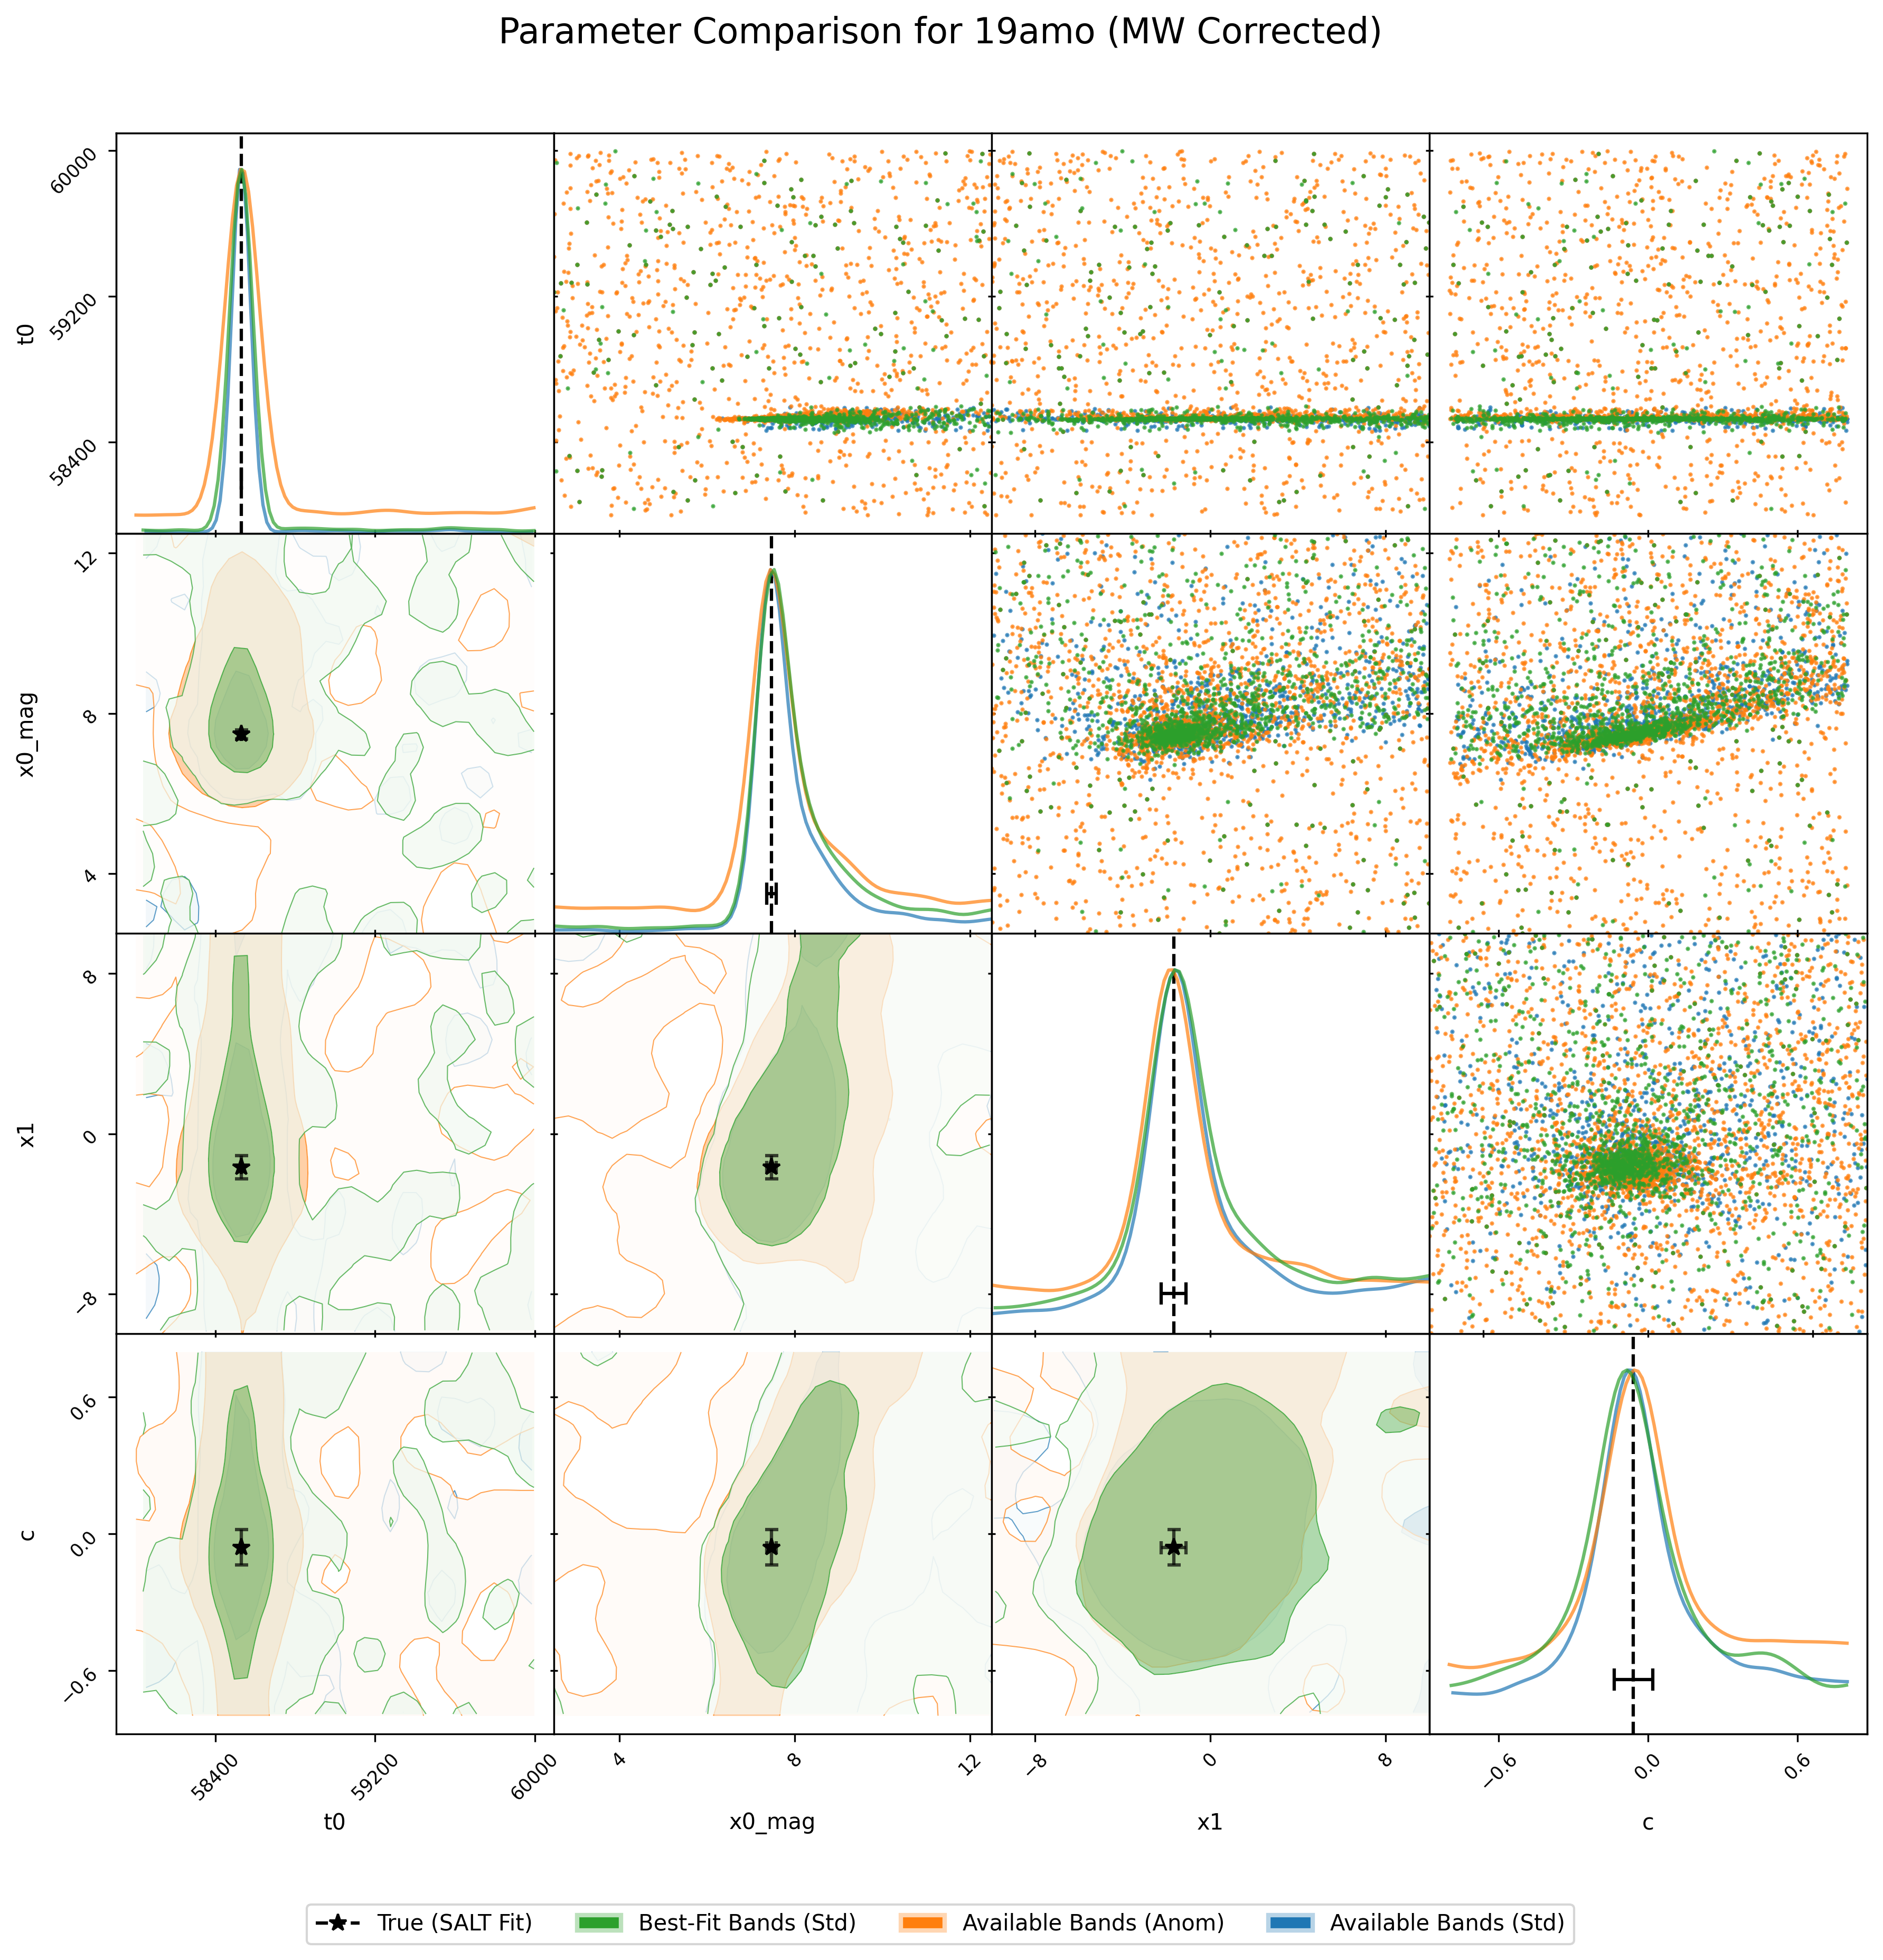
\includegraphics[width=\textwidth]{images/corner_comparison_19amo.png}
  \end{columns}
\end{frame}

\begin{frame}{SN 19vnk: Automatic filter removal}
  \begin{columns}
    \column{0.5\textwidth}
    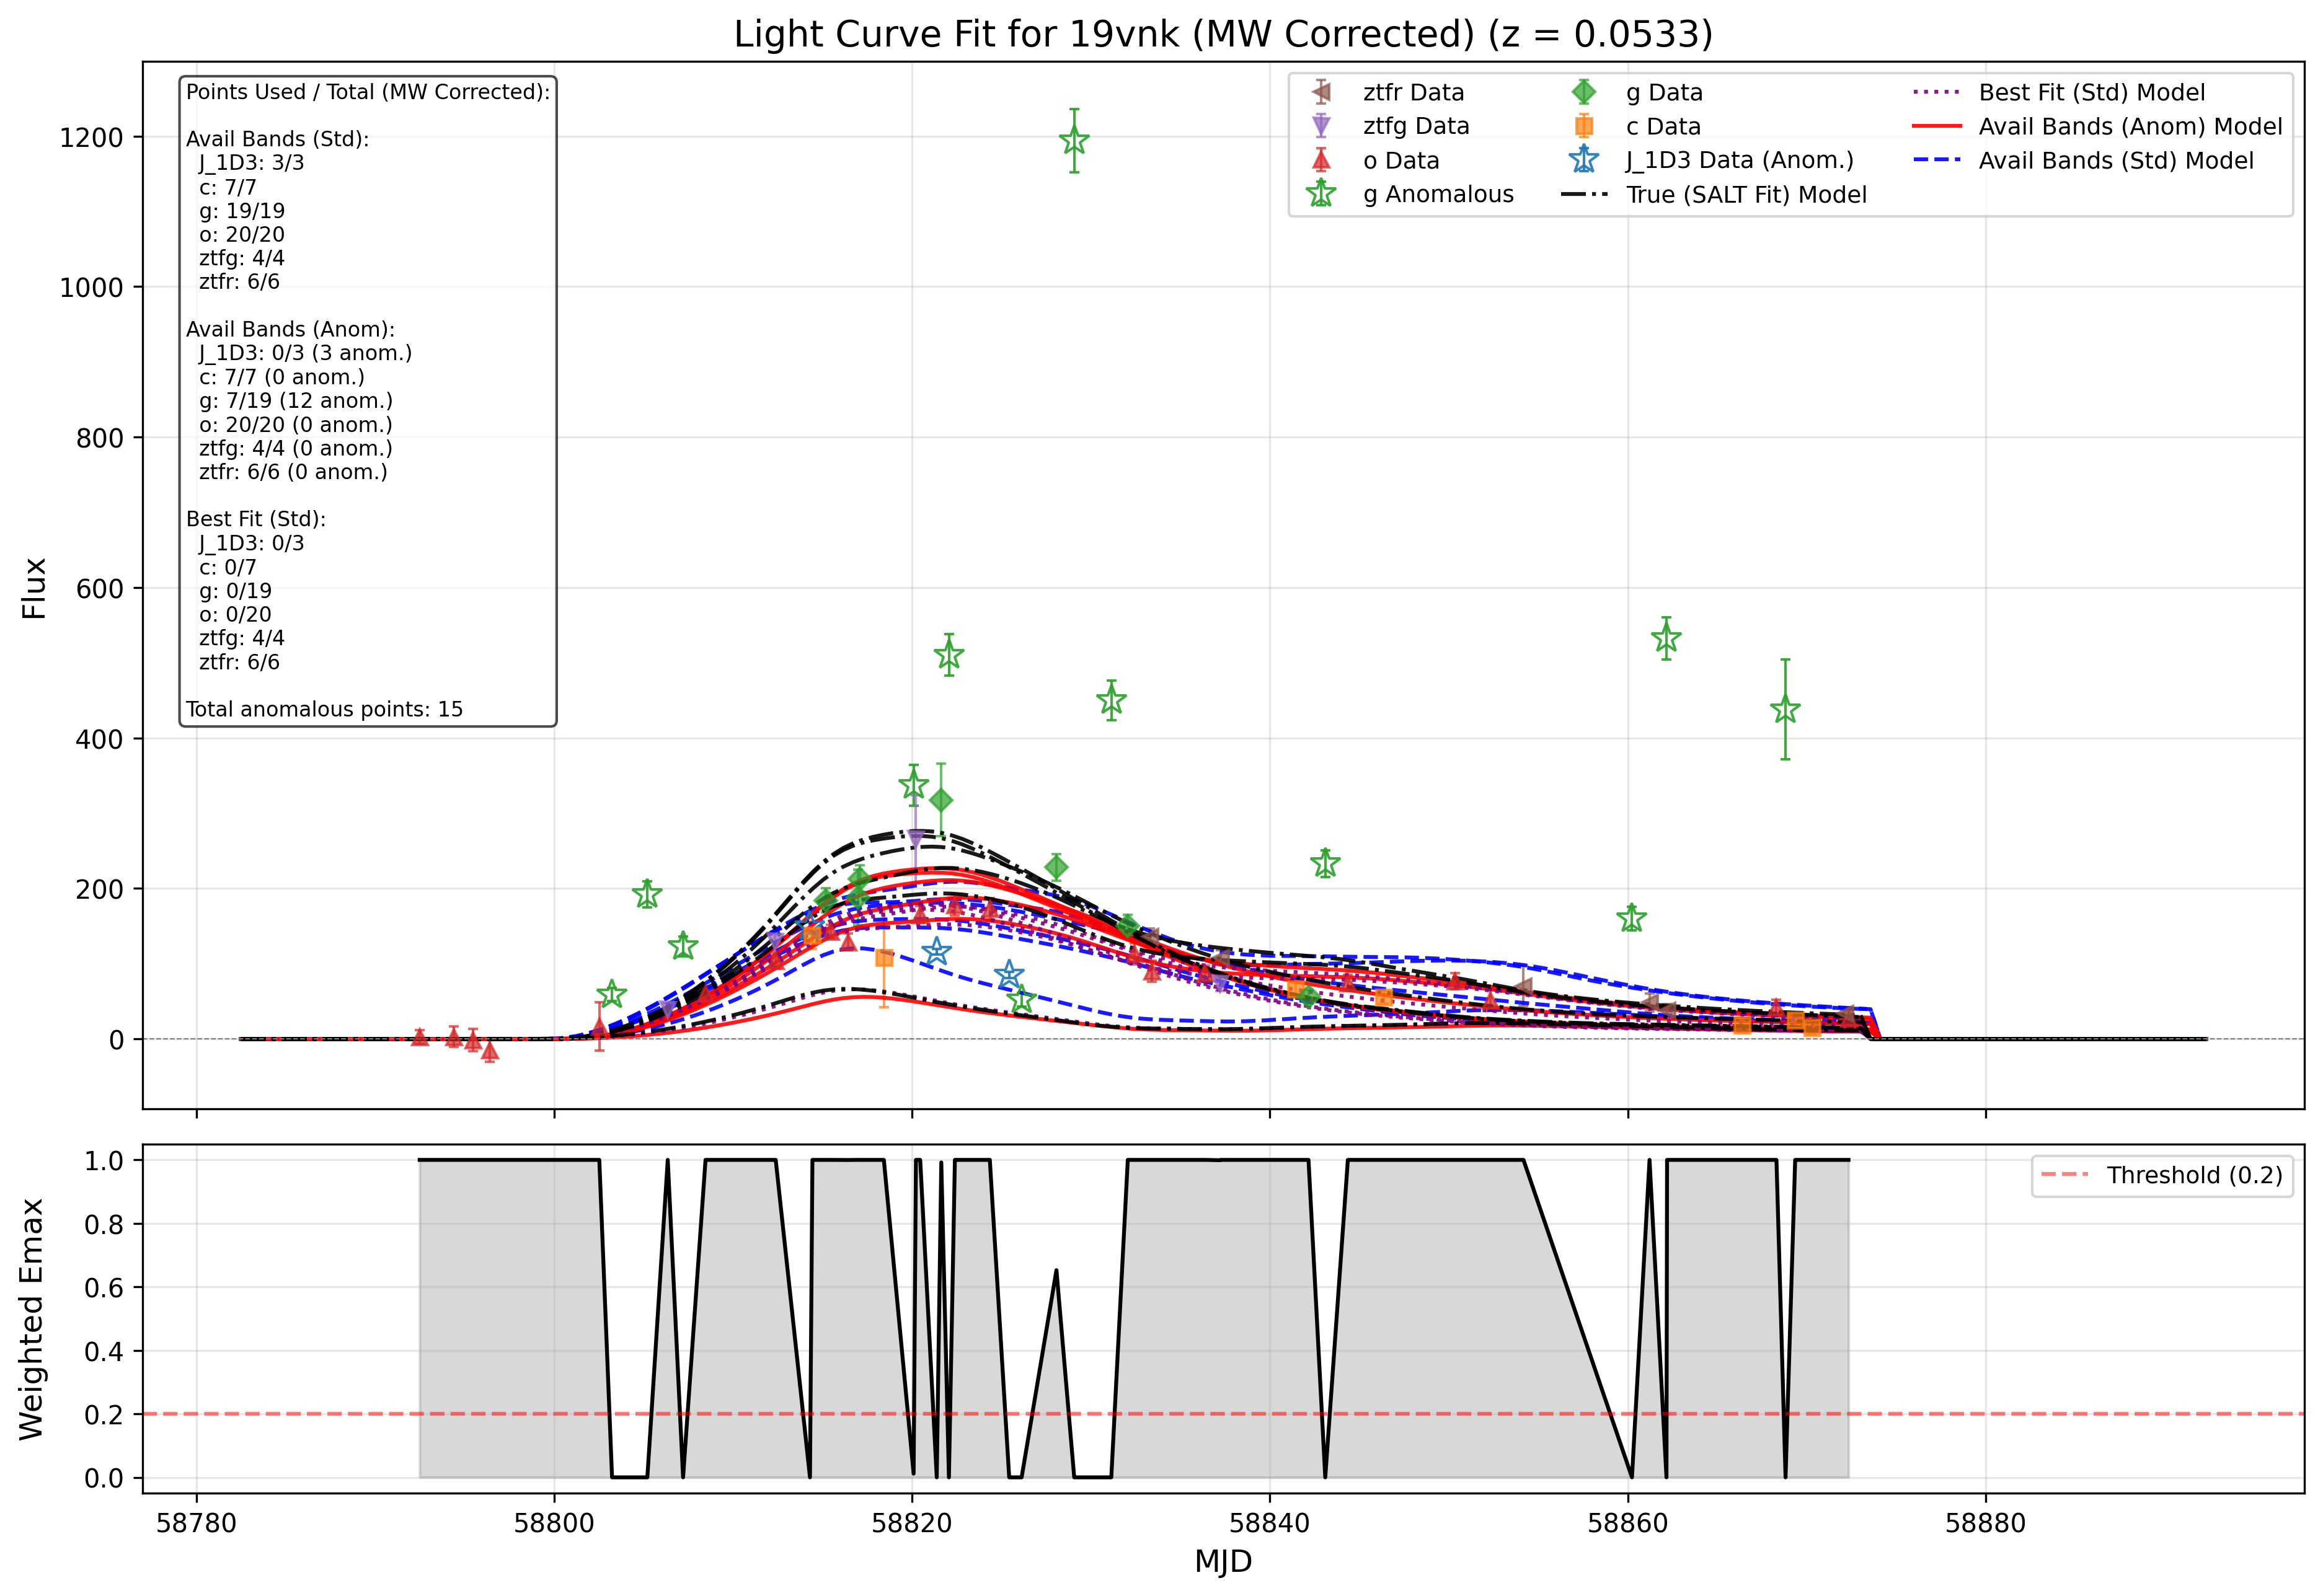
\includegraphics[width=\textwidth]{images/light_curve_comparison_19vnk.png}
    \column{0.5\textwidth}
    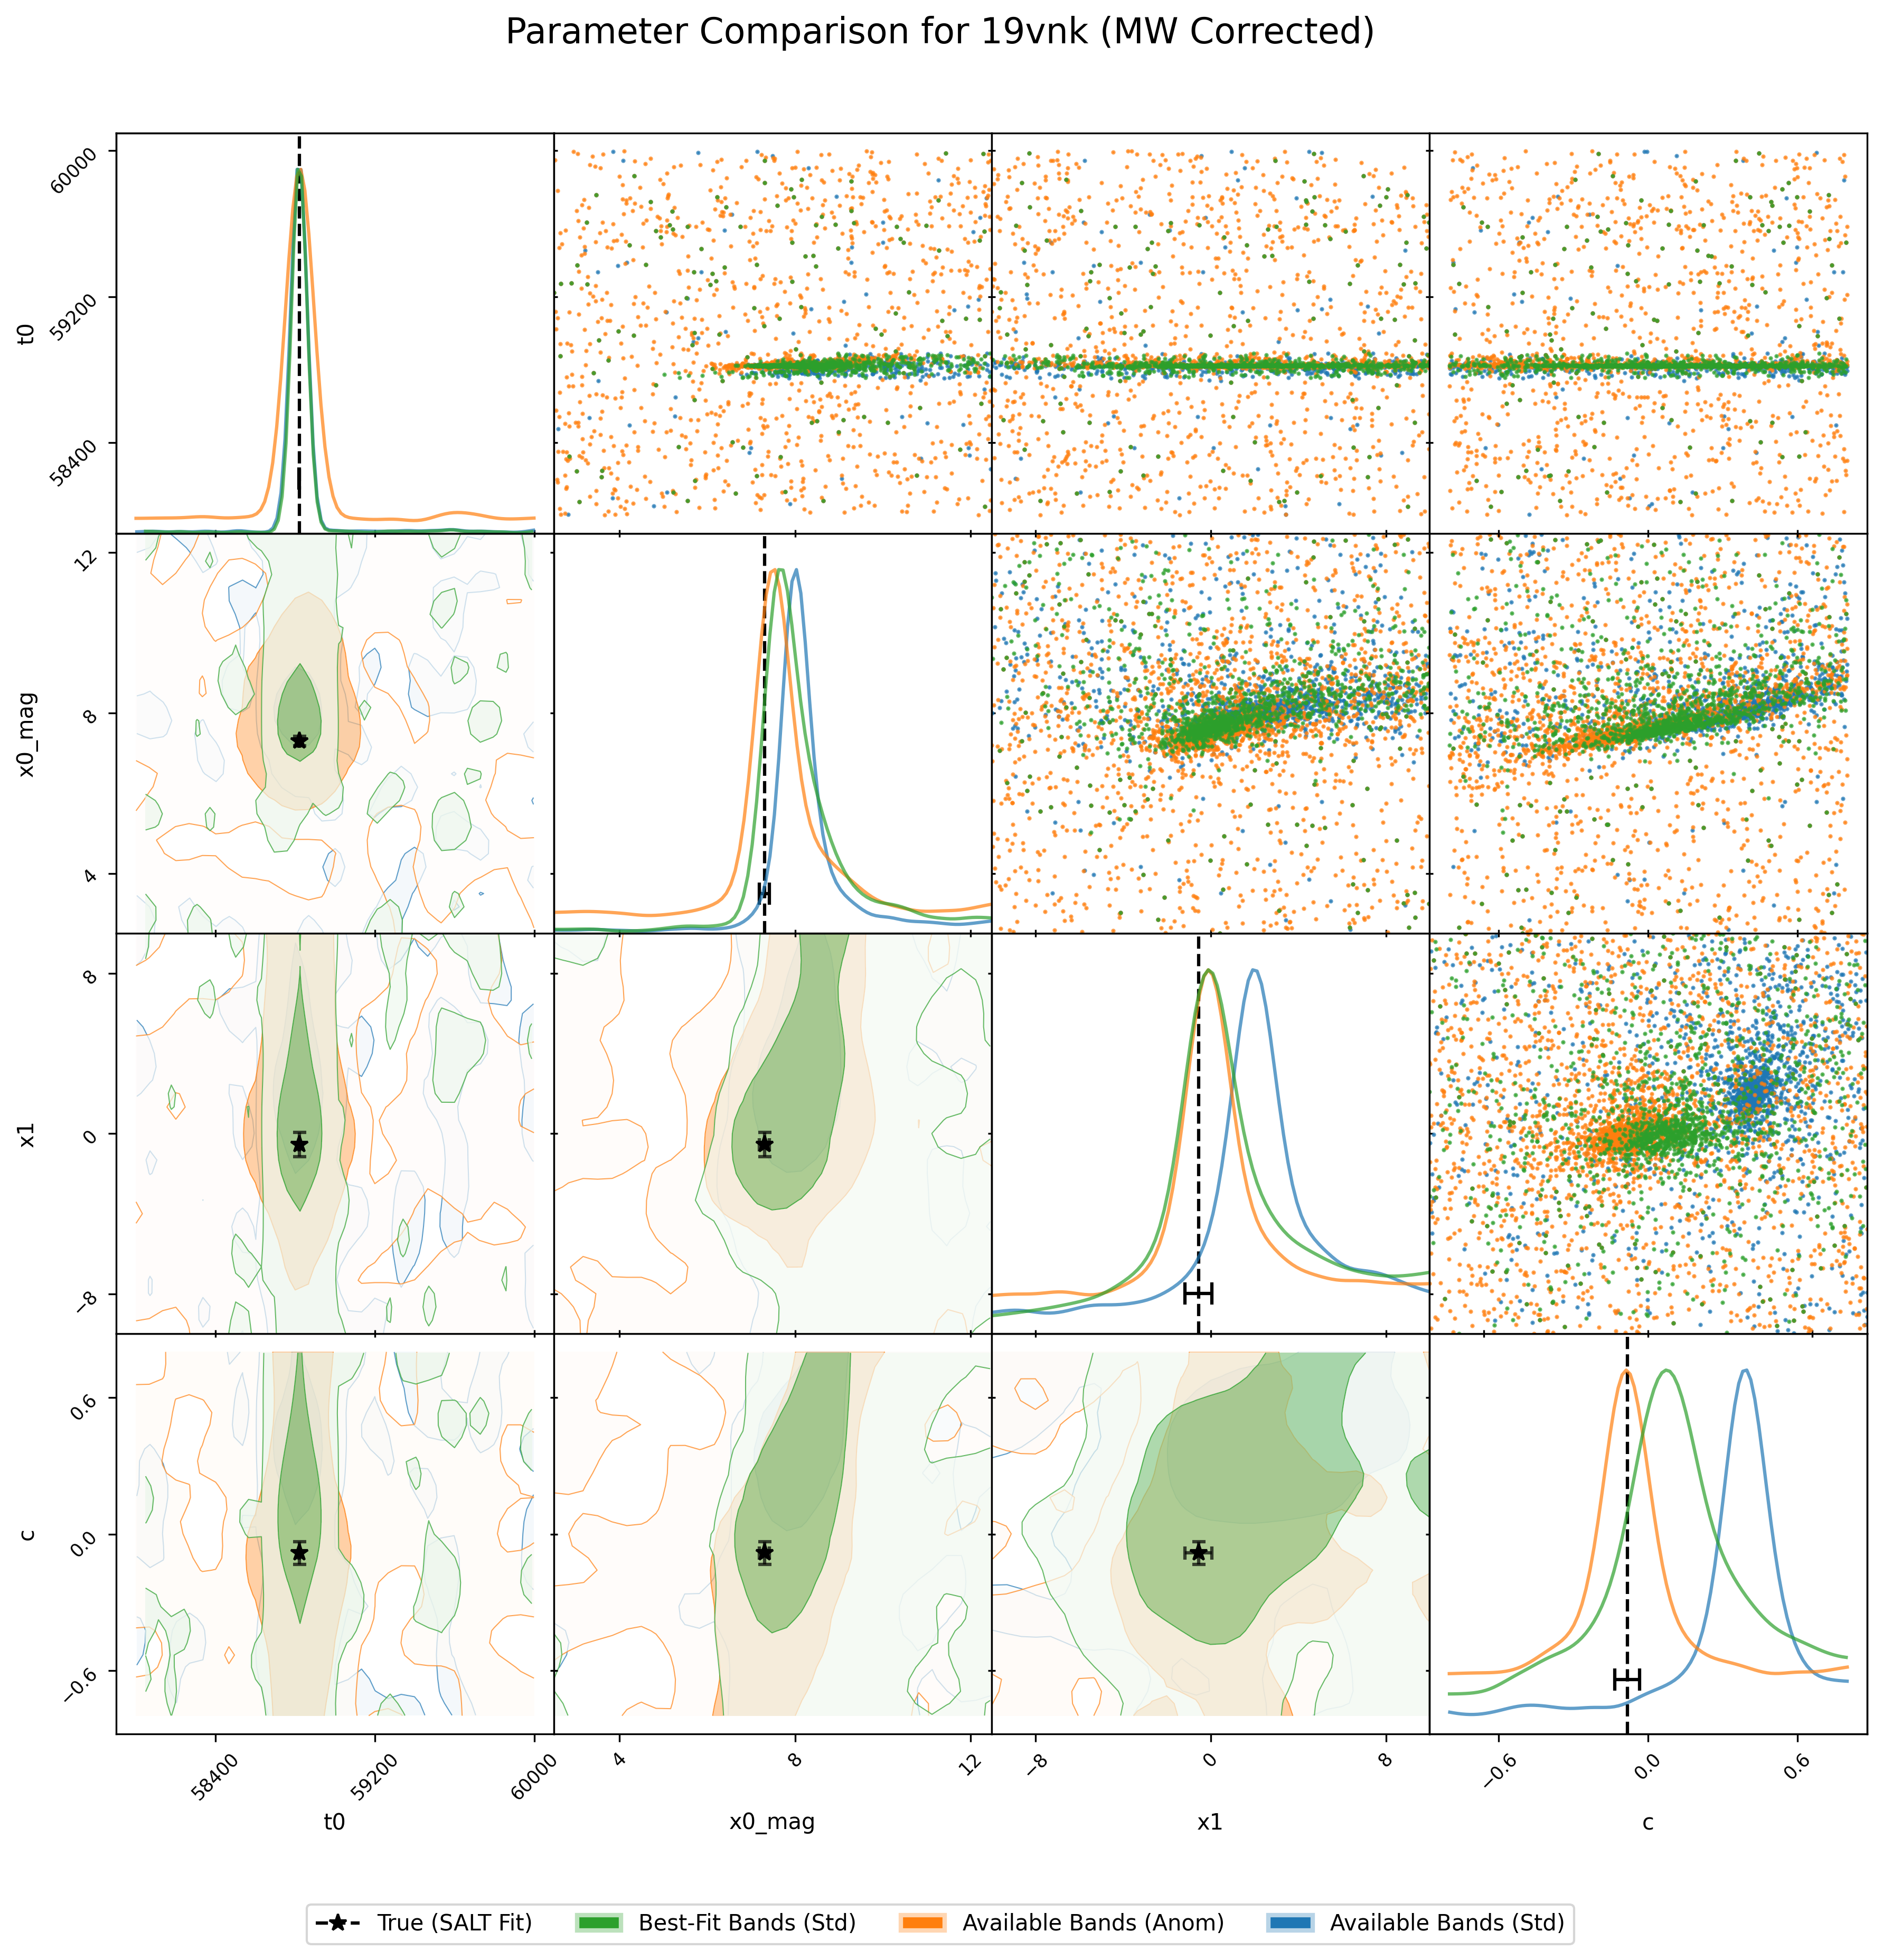
\includegraphics[width=\textwidth]{images/corner_comparison_19vnk.png}
  \end{columns}
\end{frame}

\begin{frame}{SN 19kai: Flagging while preserving some data}
  \begin{columns}
    \column{0.5\textwidth}
    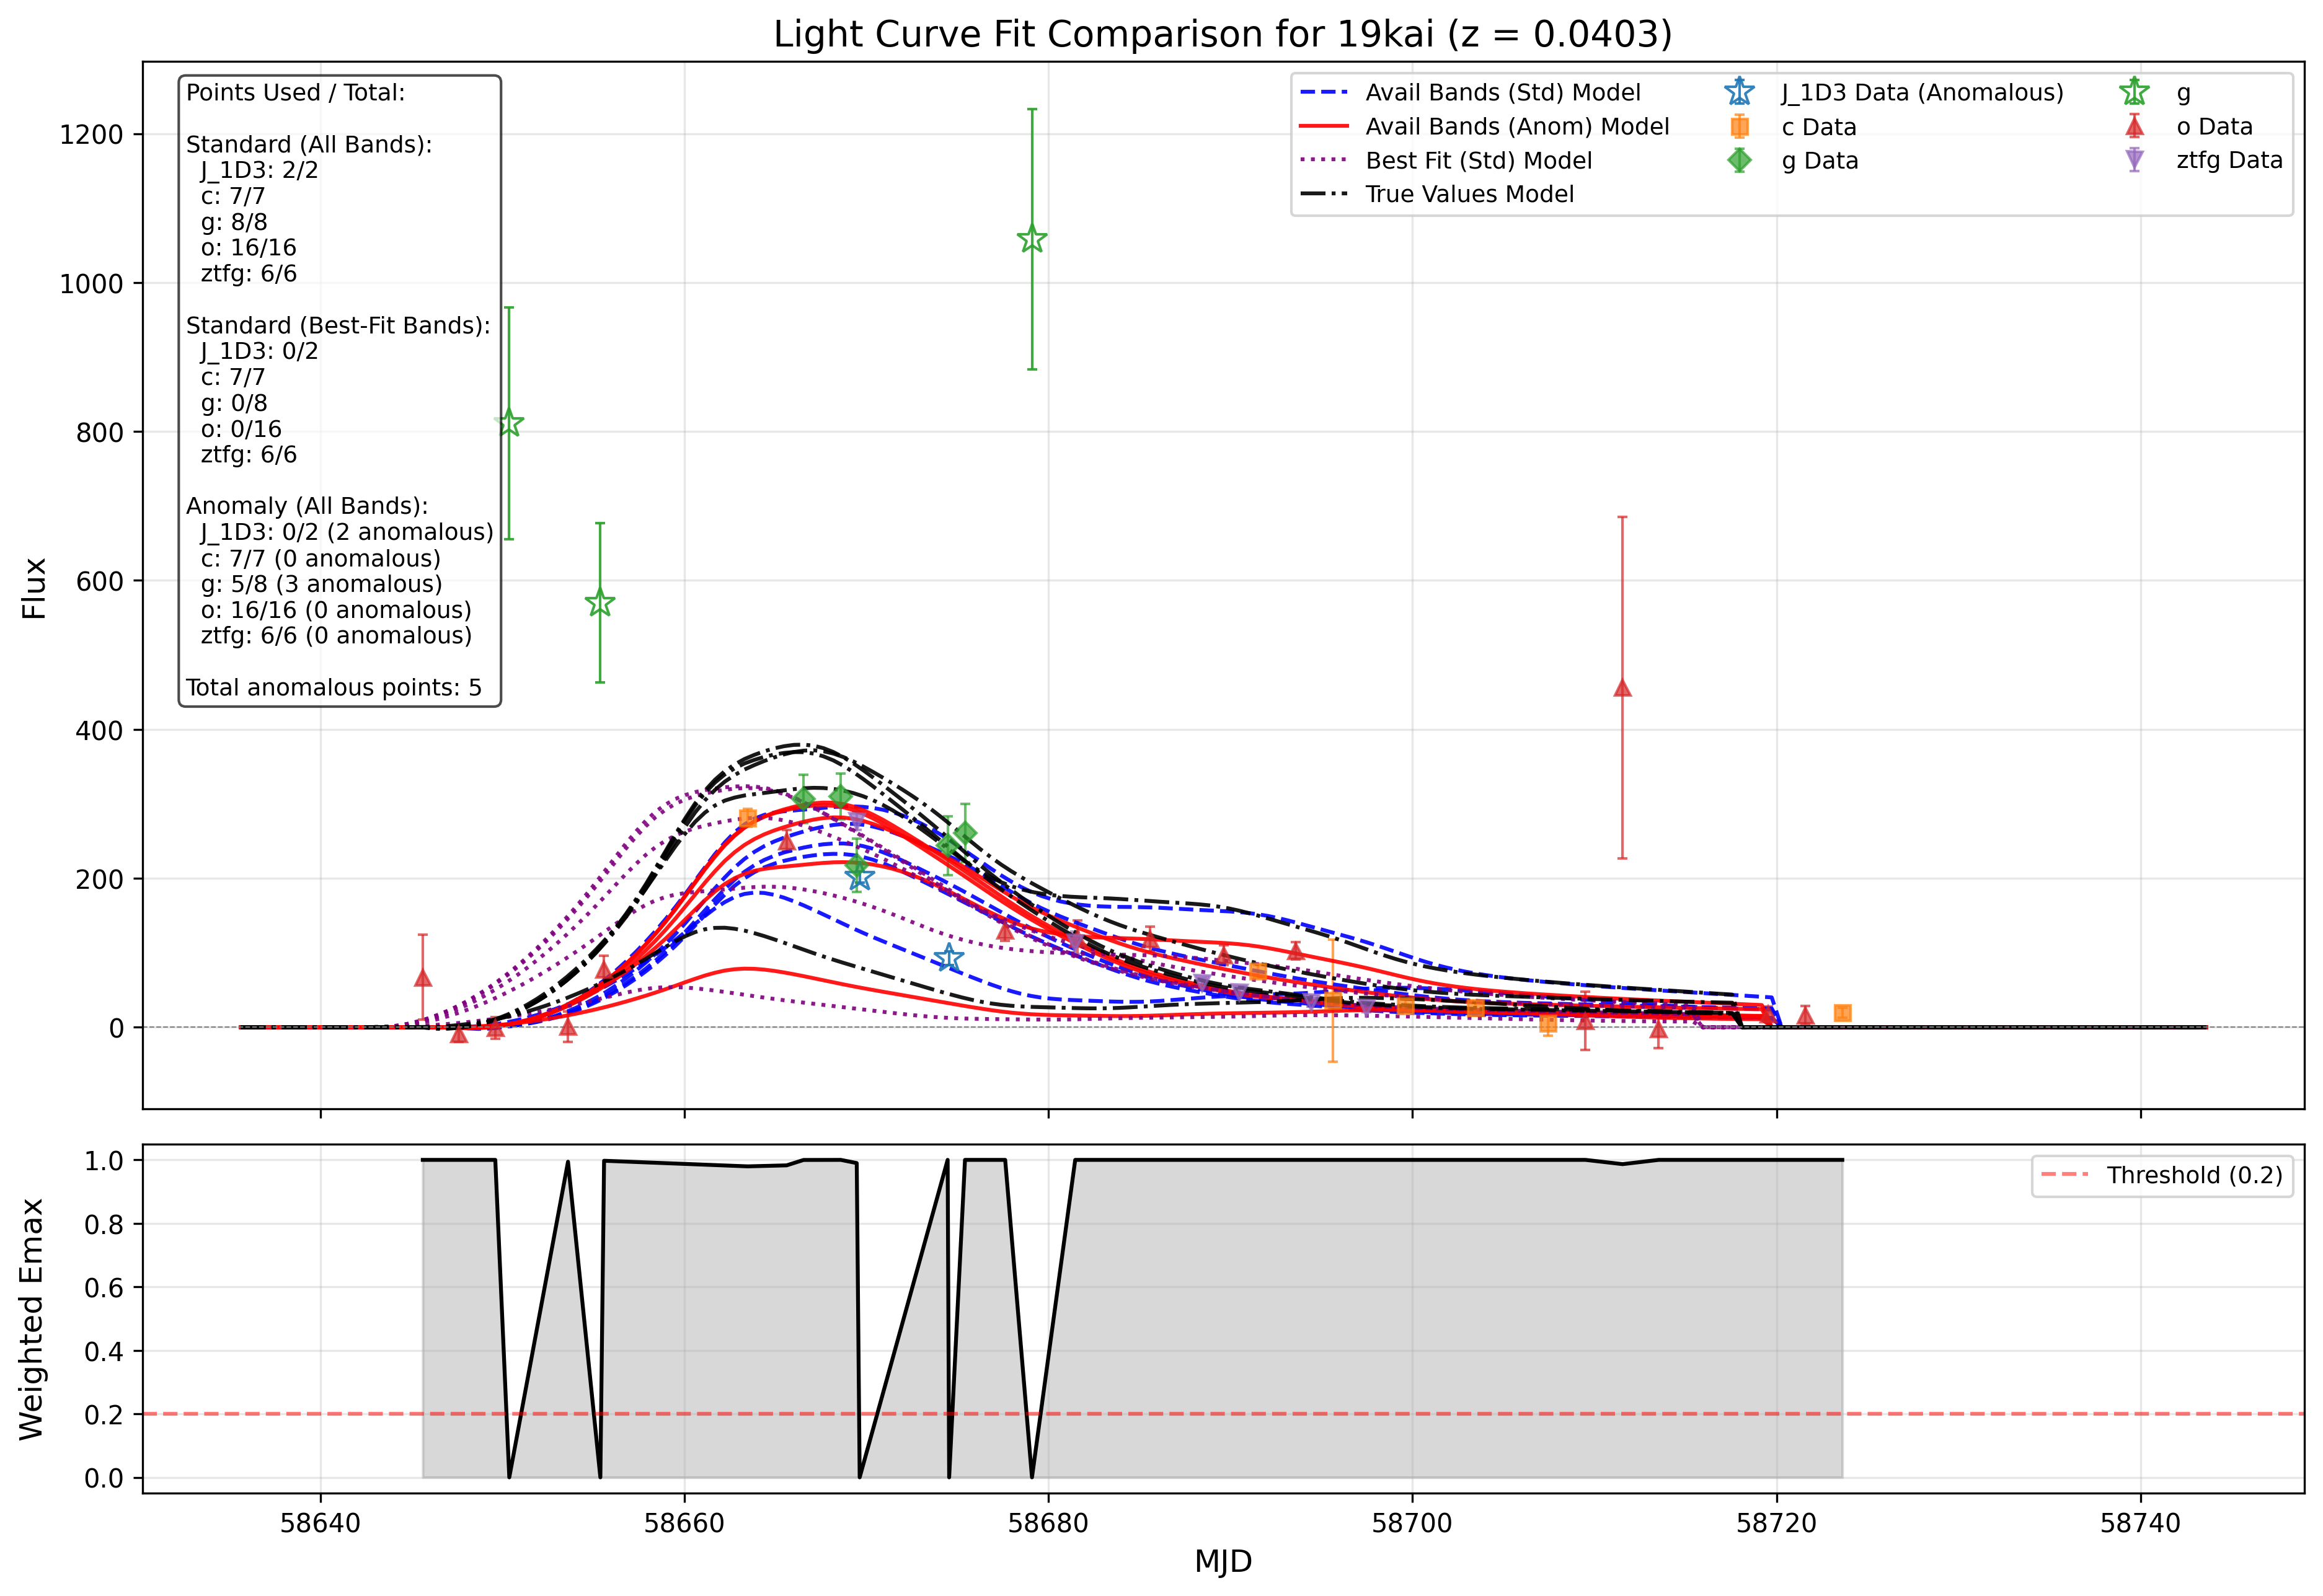
\includegraphics[width=\textwidth]{images/light_curve_comparison_19kai.png}
    \column{0.5\textwidth}
    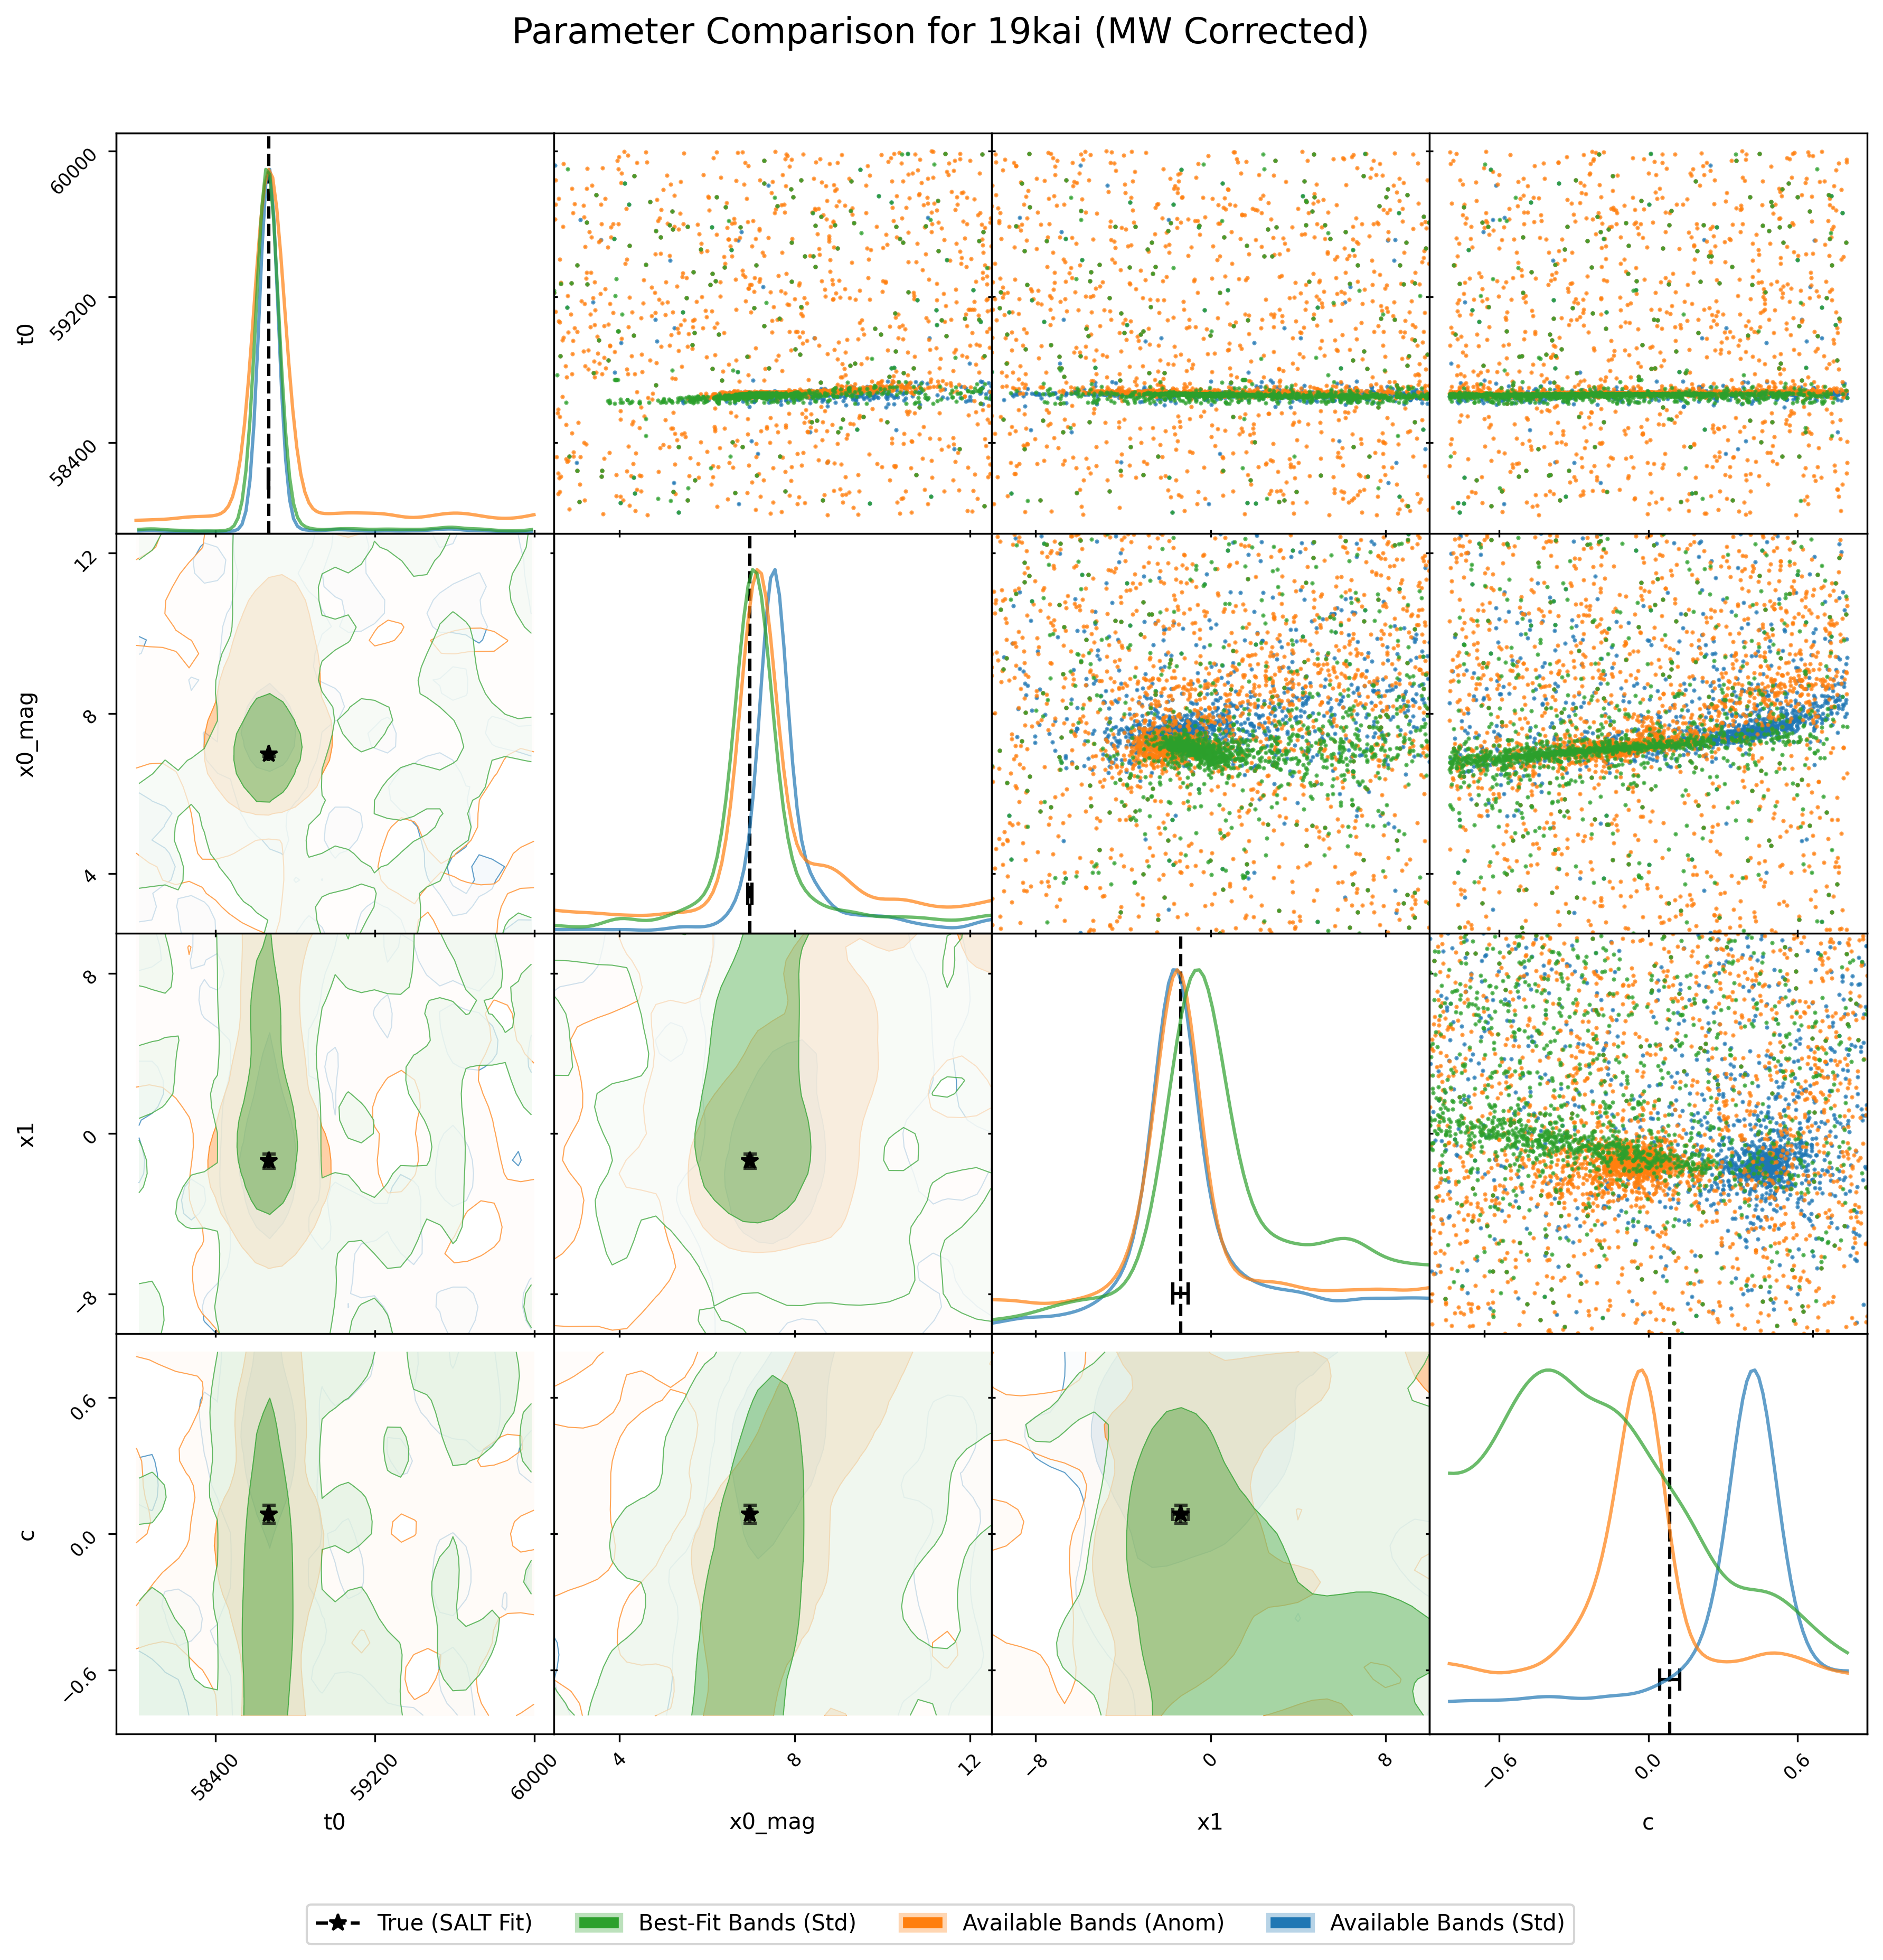
\includegraphics[width=\textwidth]{images/corner_comparison_19kai.png}
  \end{columns}
\end{frame}


\begin{frame}{SN 20aczg: Light Curve and Corner Plot Comparison}
  \begin{columns}
    \column{0.5\textwidth}
    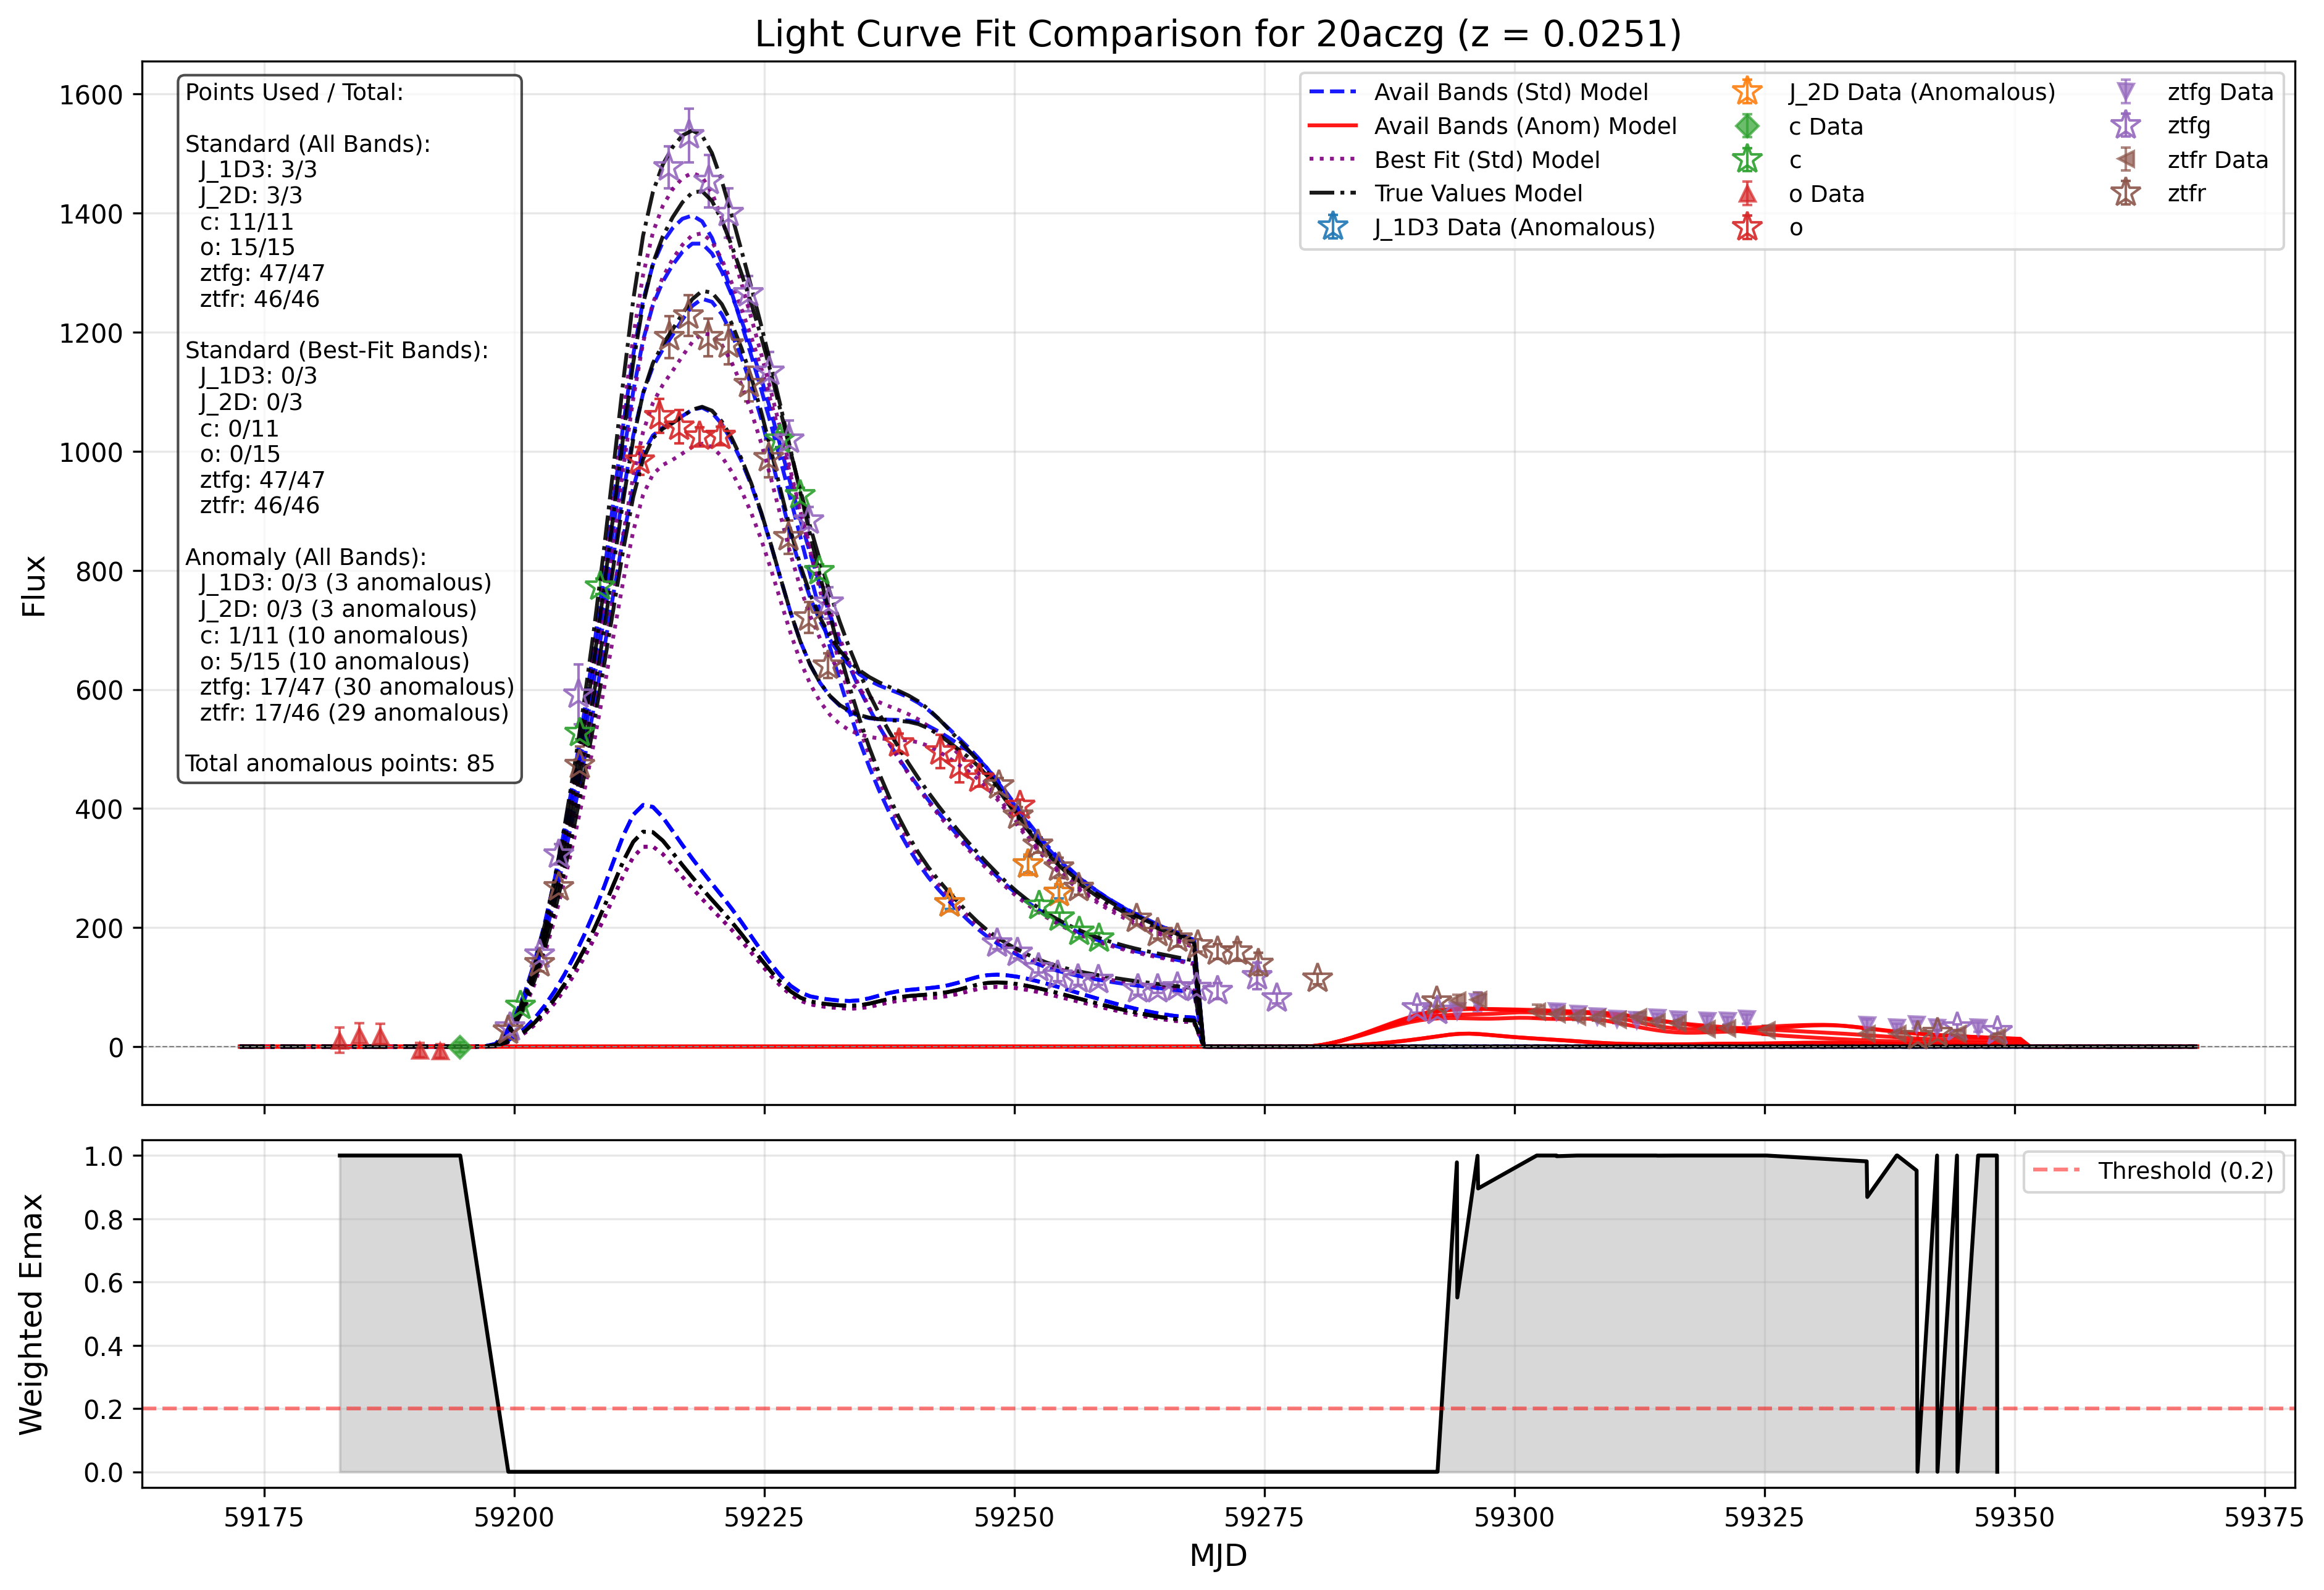
\includegraphics[width=\textwidth]{images/light_curve_comparison_20aczg.png}
    \column{0.5\textwidth}
    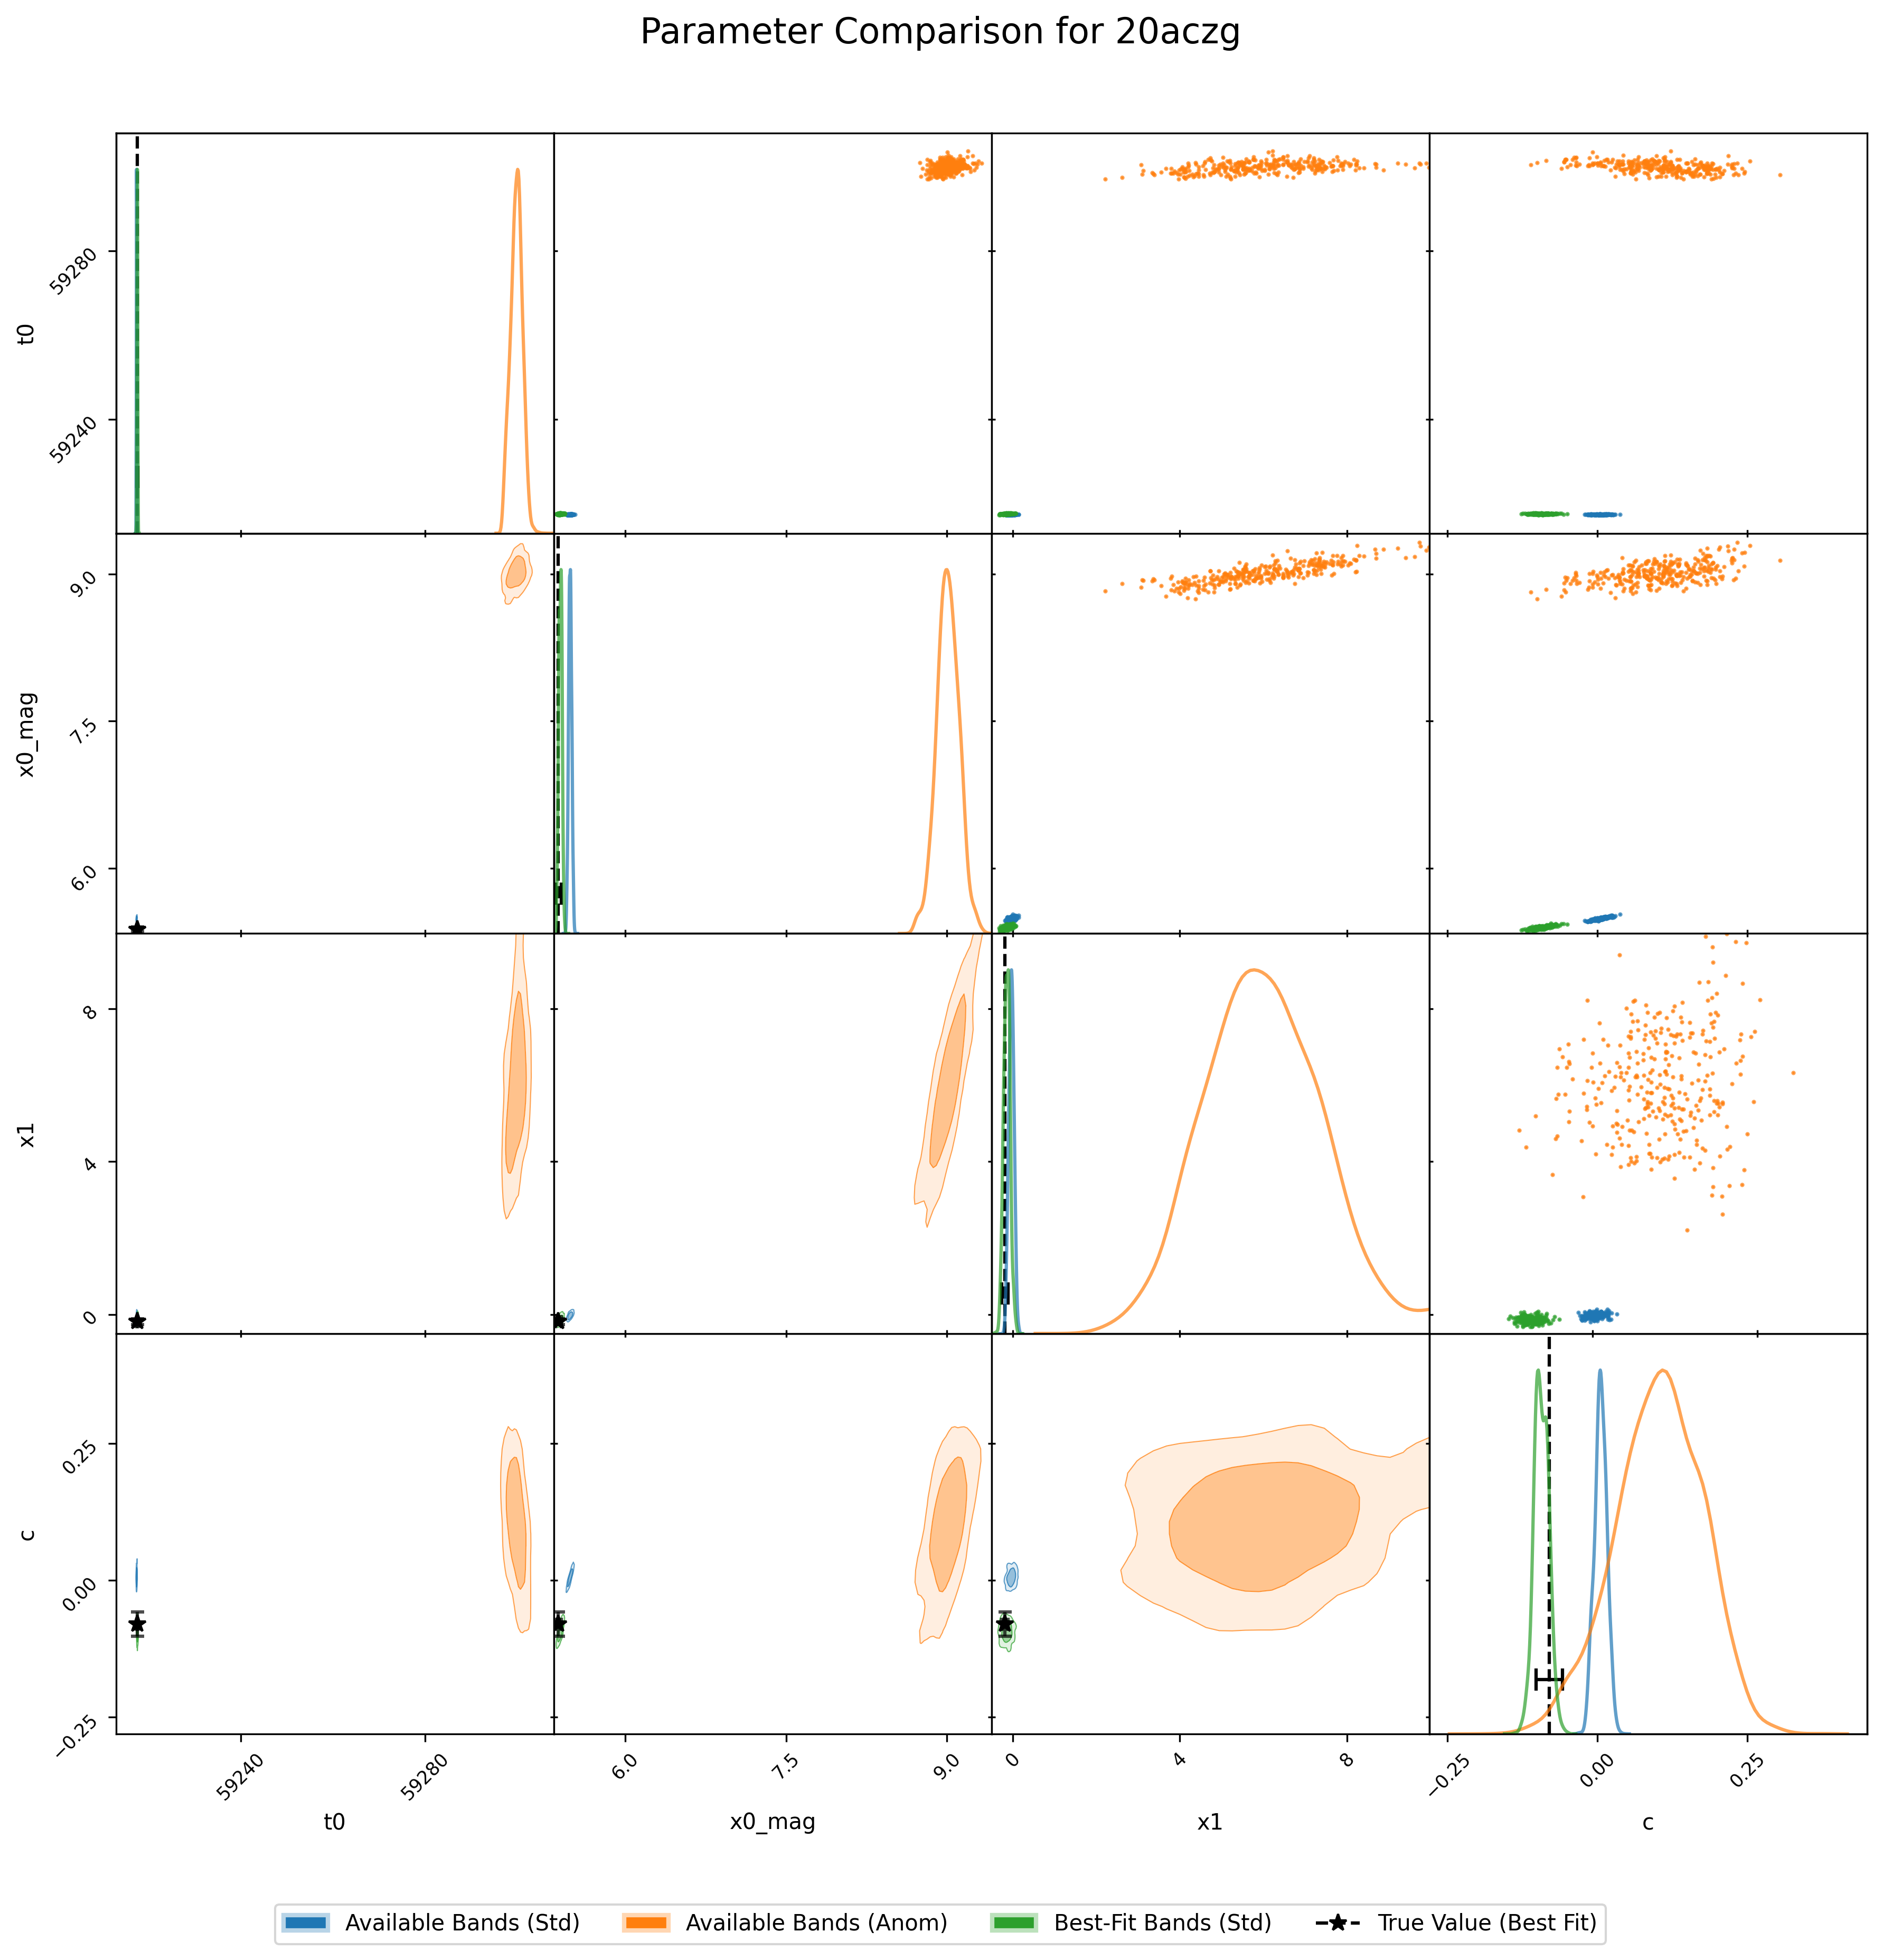
\includegraphics[width=\textwidth]{images/corner_comparison_20aczg.png}
  \end{columns}
\end{frame}

\begin{frame}{Key points}
  \begin{enumerate}
    \item Standard flagging.
  \end{enumerate}
\end{frame}

\begin{frame}{Key points}
  \begin{enumerate}
    \item Standard flagging.
    \item Automated filter selection.
  \end{enumerate}
\end{frame}

\begin{frame}{Key points}
  \begin{enumerate}
    \item Standard flagging.
    \item Automated filter selection.
    \item Data preservation from previously discarded filters.
    \item Potentially can flag non Ia automatically?
  \end{enumerate}
\end{frame}

\begin{frame}{Next steps}
  \begin{itemize}
    \item Assess Hubble diagrams 
      \begin{itemize}
        \item Quantify impact on cosmological parameter estimation
        \item Compare with traditional outlier rejection methods
        \item Evaluate systematic error reduction
      \end{itemize}
    \item Try on other datasets?
      \begin{itemize}
        \item Apply to different supernova surveys (ZTF, LSST)
        \item Test with different photometric systems
        \item Evaluate performance across redshift ranges
      \end{itemize}
  \end{itemize}
\end{frame}

\end{document}